\chapter{Topological HLT development at $\sqrt{s}=13 \TeV$}
\label{ch:hlt13TeV}

Traditionally, trigger algorithms employed at hadron colliders consisted
of selecting events based on the presence of specific particles, such
as leptons or photons, above some energy threshold and isolated from
the rest of the event. In other trigger algorithms, global
event properties (such as ``sum'' quantities like the hadronic transverse energy $H_{\mathrm{T}}$
or the missing transverse energy $\MET$) were also used. 

The event selection used in modern searches for BSM physics employ new techniques, such as kinematic variables like
\MR and \Rtwo, that no longer map on to these traditional trigger
requirements. Fortunately, the flexibility of
the software-based system allowed the development of dedicated trigger paths, based
on sophisticated kinematic variables and specific event topologies.

To target a broad range of new physics possibilities, we designed four different
types of triggers for use in $\sqrt{s}=13\TeV$ $\Pp\Pp$ collisions:
\begin{itemize}
\item Dijet razor trigger with hyperbolic \MR and \Rtwo requirements
  targeting the squark pair production topology;
\item Quadjet razor trigger with hyperbolic \MR and \Rtwo requirements
  targeting top-squark or gluino pair production topologies;
\item High-\Rtwo trigger targeting dijet+invisible topologies with
  large transverse momentum imbalance; and
\item Razor $\PH(\bbbar)$ trigger targeting production of Higgs boson
  decaying to a bottom quark-antiquark pair ($\PH\to\bbbar$) in
  association with a jet and possibly some missing transverse energy,
  i.e. $\PH(\bbbar)+\mathrm{jet}+\mathrm{invisible}$.
\end{itemize}

The dijet and quadjet razor triggers are broadly motivated by SUSY pair
production and represent an update and incremental improvement of the razor triggers
used in previous searches at $\sqrt{s}=8\TeV$~\cite{razor8TeV}. Both
sets of triggers are based on hyperbolic thresholds in the $(\MR,\Rtwo)$
plane, with the 2015 updated thresholds shown in
Fig~\ref{fig:hyperbolic}. The 2015 hyperbolic contours follow the
iso-probability contours $(\Rtwo+0.25)(\MR+300\GeV)=\mathrm{constant}$, derived from the background-only fit to the MultiJet category
in the 8\TeV razor search performed using 2012 data. This implies that
these hyperbolic contours efficiently reject background, while
maintaining a large acceptance for SUSY signal models with a large
characteristic mass scale $M_{\Delta}\gtrsim 500 \GeV$ and sufficient
transverse momentum imbalance. Another update is that the 13 \TeV razor triggers are based on PF-reconstructed objects rather
than Calo jets and muons, which means that the online $\Rtwo$ variable is
much more correlated with the offline $\Rtwo$ variable, which is also
PF-based. This leads to an improved trigger efficiency plateau of
$97\%$ for 2015 (compared to $95\%$ in 2012), shown in Fig.~\ref{fig:turnons}.

\begin{figure}[htb!]
\centering
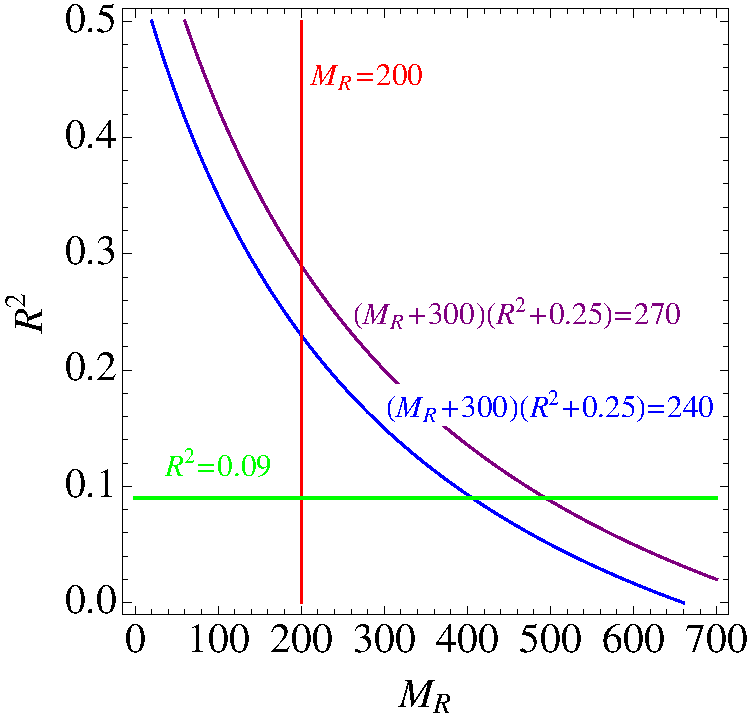
\includegraphics[width=0.8\textwidth]{figs/hlt13TeV/HLTRsqMR.pdf}
\caption{\label{fig:hyperbolic} Hyperbolic and baseline thresholds in
  \Rtwo and \MR used in the dijet and quadjet razor triggers~\cite{jmgd}. The
  hyperbolic thresholds are of the form $(\Rtwo+0.25)(\MR+300\GeV)=\mathrm{constant}$.}
\end{figure}

\begin{figure}[ht!]
\centering
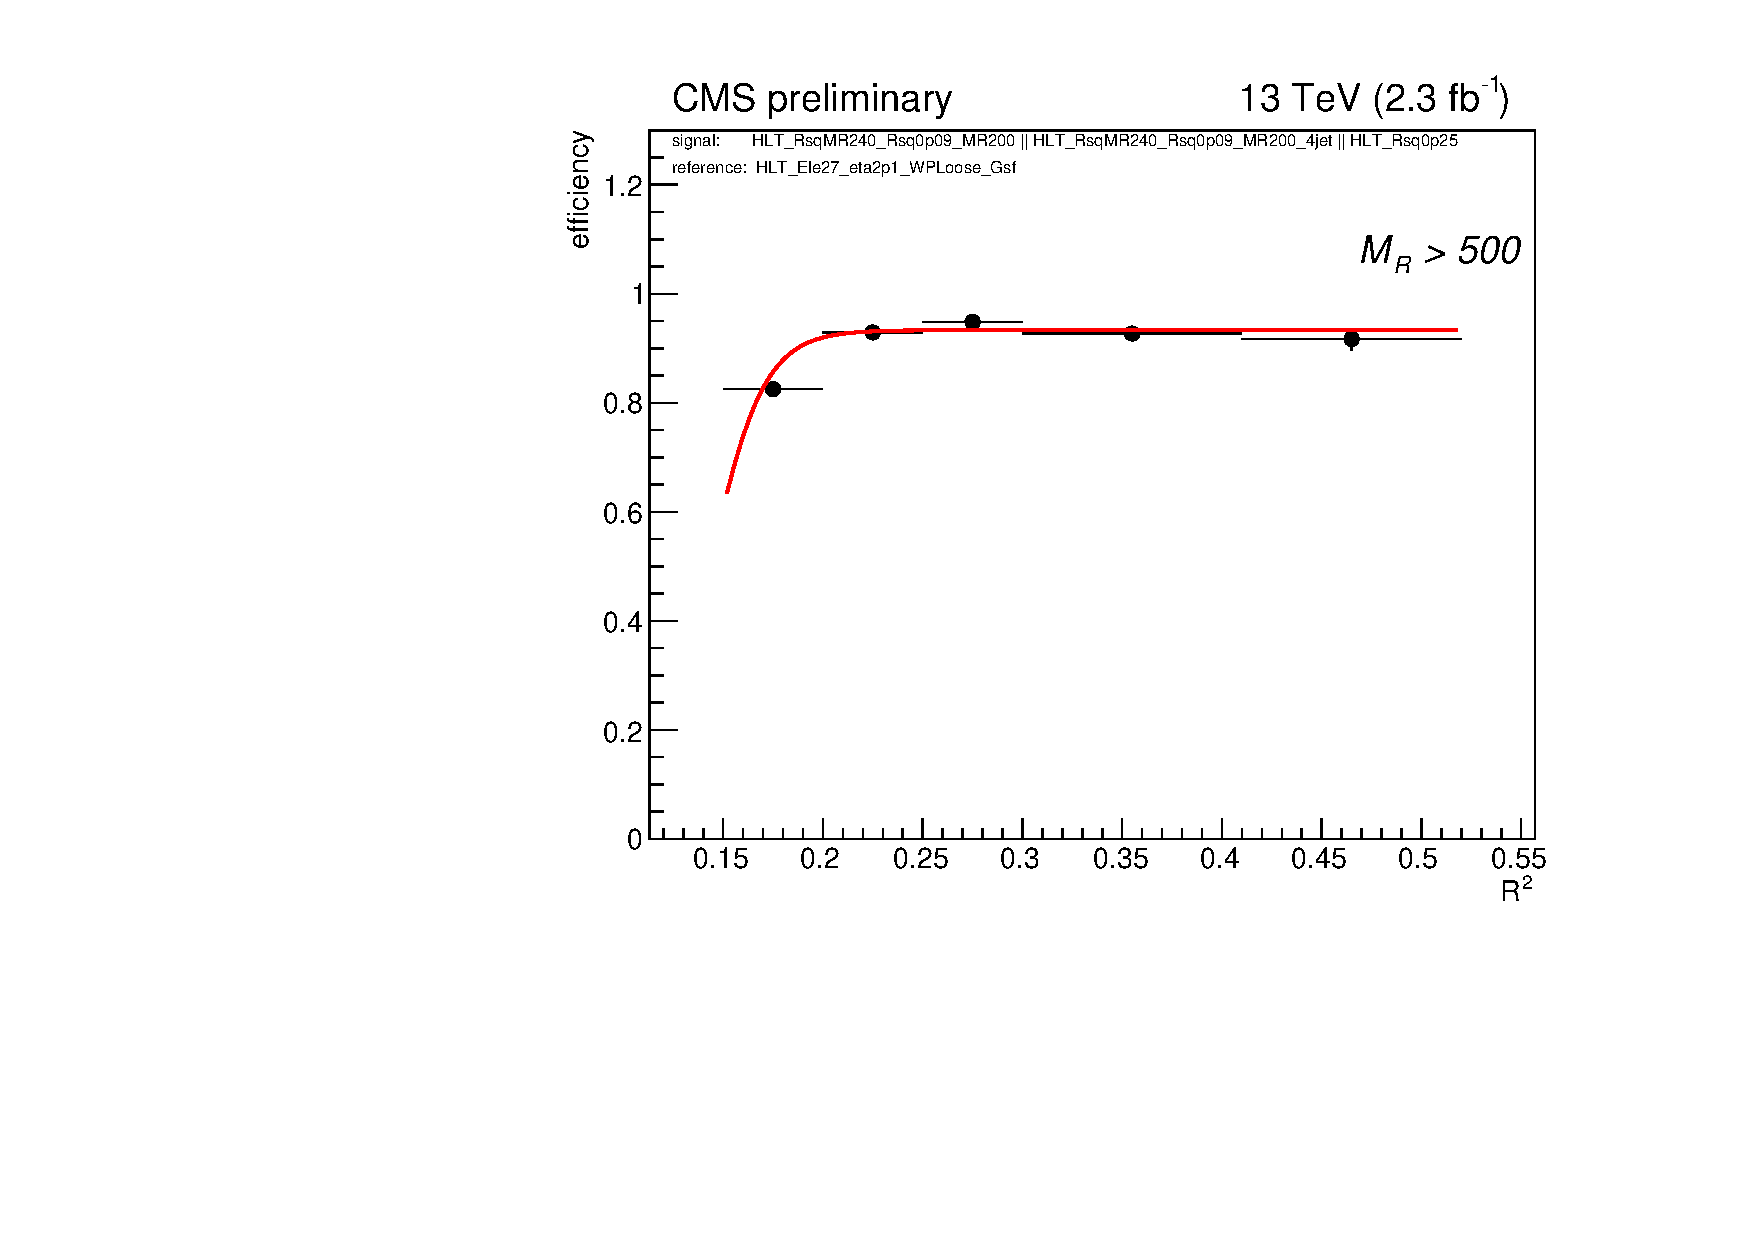
\includegraphics[width=0.7\textwidth]{figs/hlt13TeV/turnons_2015_no100GeVmuons_thesis/HLT_RsqMR240_Rsq0p09_MR200_HLT_RsqMR240_Rsq0p09_MR200_4jet_HLT_Rsq0p25_HLT_Ele27_eta2p1_WPLoose_Gsf_effRsq_MR500.pdf}
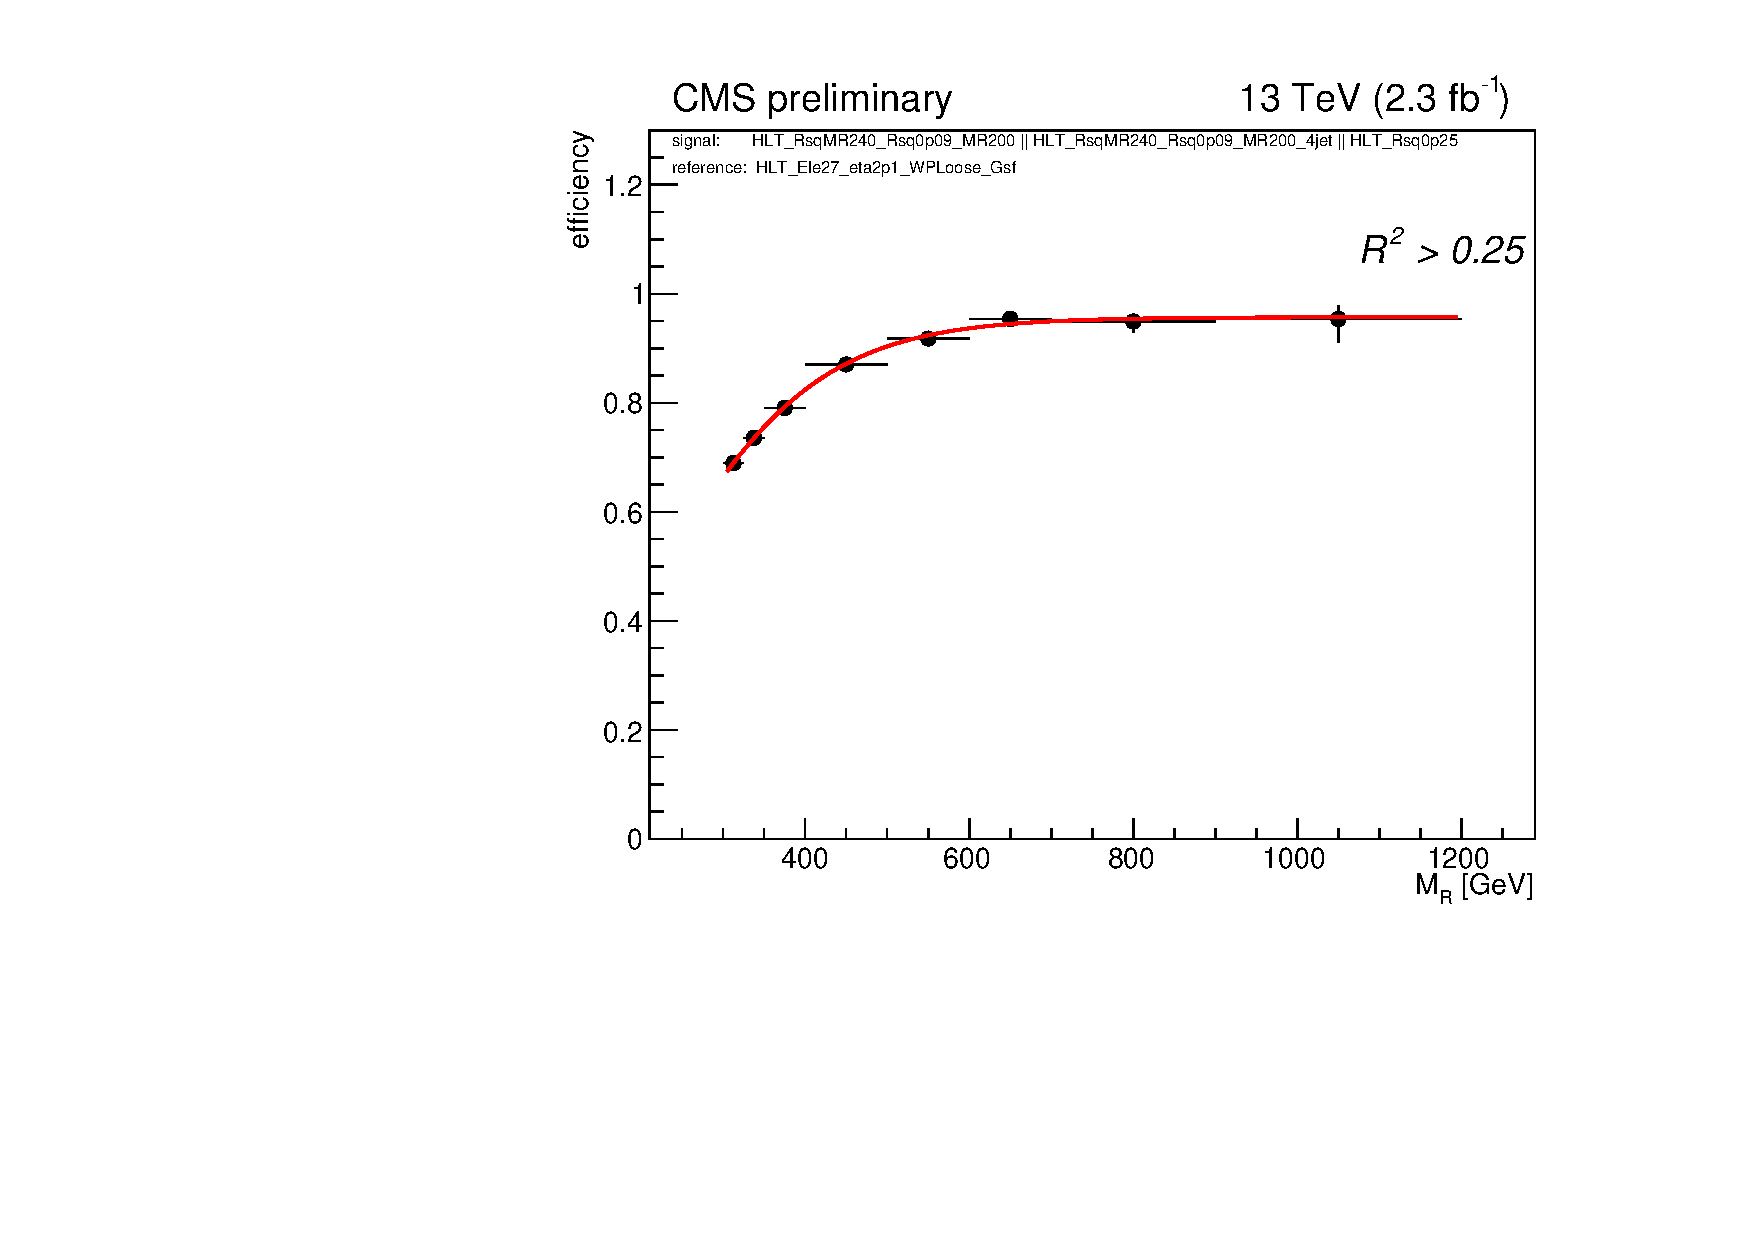
\includegraphics[width=0.7\textwidth]{figs/hlt13TeV/turnons_2015_no100GeVmuons_thesis/HLT_RsqMR240_Rsq0p09_MR200_HLT_RsqMR240_Rsq0p09_MR200_4jet_HLT_Rsq0p25_HLT_Ele27_eta2p1_WPLoose_Gsf_effMR_Rsq0p25.pdf}
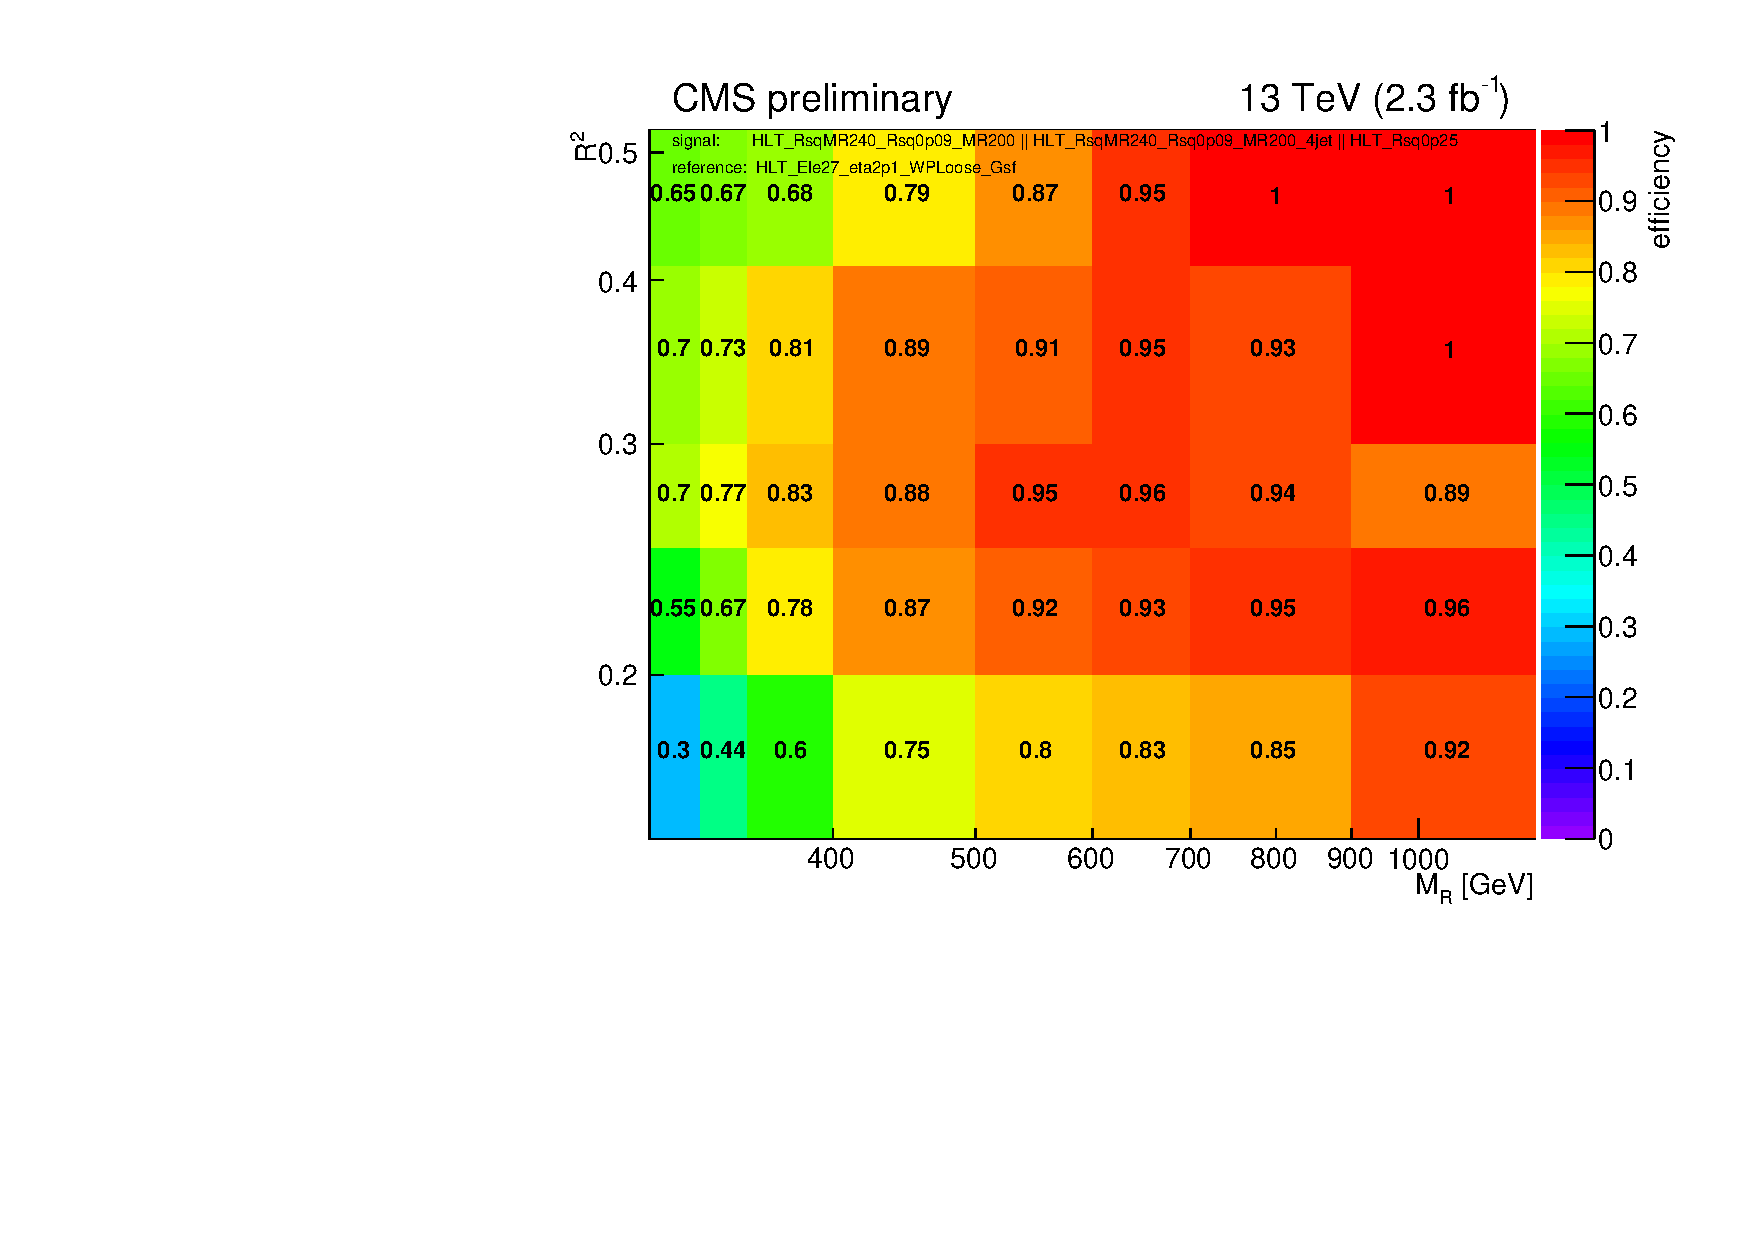
\includegraphics[width=0.7\textwidth]{figs/hlt13TeV/turnons_2015_no100GeVmuons_thesis/HLT_RsqMR240_Rsq0p09_MR200_HLT_RsqMR240_Rsq0p09_MR200_4jet_HLT_Rsq0p25_HLT_Ele27_eta2p1_WPLoose_Gsf_eff2D.pdf}
\caption{\label{fig:turnons} Trigger efficiency of the boolean ``or'' of
  the dijet, quadjet and high-\Rtwo triggers as used in the search of
  Ch.~\ref{ch:analysis13TeV}, measured in a data sample of
  single-electron events as a function of $\Rtwo$ (top), $\MR$ (middle), and as a function of $(\MR,\Rtwo)$ (bottom)~\cite{jmgd}.}
\end{figure}

The high-\Rtwo trigger is motivated by the search for the direct
production of dark matter (DM) particles at the
LHC~\cite{Khachatryan:2016reg}.  DM particles themselves
would not leave a detectable signal in the detector, but if
they were produced in association with high-energy quarks or gluons,
they could produce signatures with jets and transverse
momentum imbalance. The traditional approach, employed by both CMS and
ATLAS, is to search in events with one high-$\pt$ jet and large $\MET$
(so-called monojet searches)~\cite{Aad:2011xw,Chatrchyan:2012me}. A complementary
approach is to search in events with at least two jets passing a looser
event selection using the razor variables. The sensitivity of these variables to direct DM production was
suggested in Ref.~\cite{Fox:2012ee}, and the search carried out by CMS
demonstrates that the resulting sensitivity is comparable to that of
monojet searches~\cite{Fox:2012ee,Papucci:2014iwa,Khachatryan:2016reg}.
The hallmark of many direct DM production models in the razor plane is
a peaking behavior near $\Rtwo\gtrsim 0.8$ and an exponentially
falling $\MR$ distribution with no special structure. For this reason,
the high-\Rtwo trigger is designed with a threshold in \Rtwo but no
requirement on \MR to allow for greater DM signal acceptance.

Finally, the razor $\PH(\bbbar)$ trigger is motivated by an
excess observed in Run 1 by CMS in events with a Higgs boson decaying
to two photons ($\PH\to\Pgg\Pgg$) plus at least one extra jet~\cite{RazorHgaga}. The excess,
corresponding to a local significance of
$2.9\sigma$, consists of five events observed with $400\GeV<\MR<1400
\GeV$,  $\Rtwo>0.05$, and $m_{\Pgg\Pgg}$ consistent with $m_\PH= 125
\GeV$ in a high-resolution diphoton category, compared to less than one
expected background event. The general idea is to search for a similar
signature in the $\PH\to\bbbar$ channel, which comes with a larger
signal yield (90,000 times more assuming SM Higgs branching ratios),
but a much larger background, resulting in a considerably worse
signal-to-background ratio and a much larger background event rate. These final
two features make the definition of an optimal trigger strategy much more
challenging than in the $\PH\to\Pgg\Pgg$ decay channel. Given this, the trigger
requirements of three jets, two \cPqb-jets, $\MR>300
\GeV$, $\Rtwo>0.02$, and $m_{\bbbar}$ roughly consistent with $m_\PH= 125
\GeV$ are chosen to (a) maintain signal acceptance based on the observed
features, (b) accept additional events outside of the $m_\PH$ window
to permit a robust background estimation based on a fit, and (c)
limit the rate and average CPU time of the trigger to an acceptable
level.

For each trigger, we developed two different versions: a ``main''
version intended for $7\times 10^{33}$ cm$^{-2}$ s$^{-1}$ and 20 average
pileup interactions, and a ``backup'' version, with tighter thresholds
intended for $1.4\times 10^{34}$ cm$^{-2}$ s$^{-1}$ and 40 average
pileup interactions. The correspondence between the purpose of each
trigger and its path name is shown in Tab.~\ref{tab:pathnames}. Each trigger path name encodes the main
  selection criteria. For the dijet and quadjet triggers, ``RsqMR240'' denotes the hyperbolic
  threshold $(\Rtwo+0.25)(\MR+300\GeV)=240\GeV$, ``Rsq0p09\_MR200''
  denotes the baseline thresholds $\Rtwo>0.09$ and $\MR>200\GeV$, and ``4jet'' denotes a
  four-jet requirement where the two leading (remaining) jets are required to have
  a minimum $\pt$ of $50\GeV$ ($40\GeV$). For the $\PH(\bbbar)$
  trigger, ``TriPFJet80\_60\_40'' denotes a three-jet requirement where the
  leading, subleading, and remaining jet is required have a
  minimium \pt of $80\GeV$, $60\GeV$, and $40\GeV$, respectively, 
``DoublePFBTagCSV0p7\_0p4'' denotes a two \Pqb-tagged jet
  requirement, with CSV discriminator values above 0.7 and 0.4,
  respectively, and ``Mbb60\_200'' denotes the
  $60<m_{\bbbar}<200\GeV$ mass window.

\begin{table*}[ht!]
\centering
 \caption{Correspondence between the purpose of each
trigger and its path name.\label{tab:pathnames}}
\resizebox{\textwidth}{!}{
\begin{tabular}{l|l}
\hline\hline
Trigger path  & Purpose \\
\hline
HLT\_RsqMR240\_Rsq0p09\_MR200 & main dijet trigger\\
HLT\_RsqMR270\_Rsq0p09\_MR200 & backup dijet trigger \\
HLT\_RsqMR240\_Rsq0p09\_MR200\_4jet & main quadjet trigger \\
HLT\_RsqMR270\_Rsq0p09\_MR200\_4jet & backup quadjet trigger \\
HLT\_Rsq0p25 & main high-\Rtwo trigger \\
HLT\_Rsq0p30 & backup high-\Rtwo trigger \\ 
HLT\_Rsq0p02\_MR300\_TriPFJet80\_60\_40\_&\multirow{2}{*}{main $\PH(\bbbar)$ trigger} \\
~DoublePFBTagCSV0p7\_0p4\_Mbb60\_200 & \\
HLT\_Rsq0p02\_MR300\_TriPFJet80\_60\_40\_ & \multirow{2}{*}{backup $\PH(\bbbar)$ trigger}  \\
~DoublePFBTagCSV0p7\_Mbb60\_200 & \\
\hline\hline
\end{tabular}}
\end{table*}

\section{HLT path design}

The design of the four main HLT paths in terms of producers (in
purple) and filters (in blue) is shown
in Fig.~\ref{fig:HLTdesign}. The first step is always a filter, which
rejects events with no hadronic activity above a certain threshold reconstructed by the L1 trigger.
As detailed in Sec.~\ref{sec:trigger}, there are two main technical
constraints an HLT path must satisfy: (a) the average CPU time required must be
small enough so that the entire HLT menu fits within the timing budget
 of $\sim160$ \unit{ms} per event and (b) the rate must
be small enough so that the entire HLT menu fits within the maximum
allowable rate  of $\sim1$ \unit{kHz}. To satisfy the timing
requirement, all the paths are outfitted with
calorimetric prefilters. The aim of these prefilters is to reject
events based only on information from the calorimeters, whose
reconstruction algorithms are much faster than the PF algorithm. In
other words, to keep the timing of the paths manageable, it is
necessary to limit the input rate to the PF algorithm. Thus, all four
triggers have a prefilter based on calorimeter-based versions of the razor
variables.

\begin{figure}[ht!]
\centering
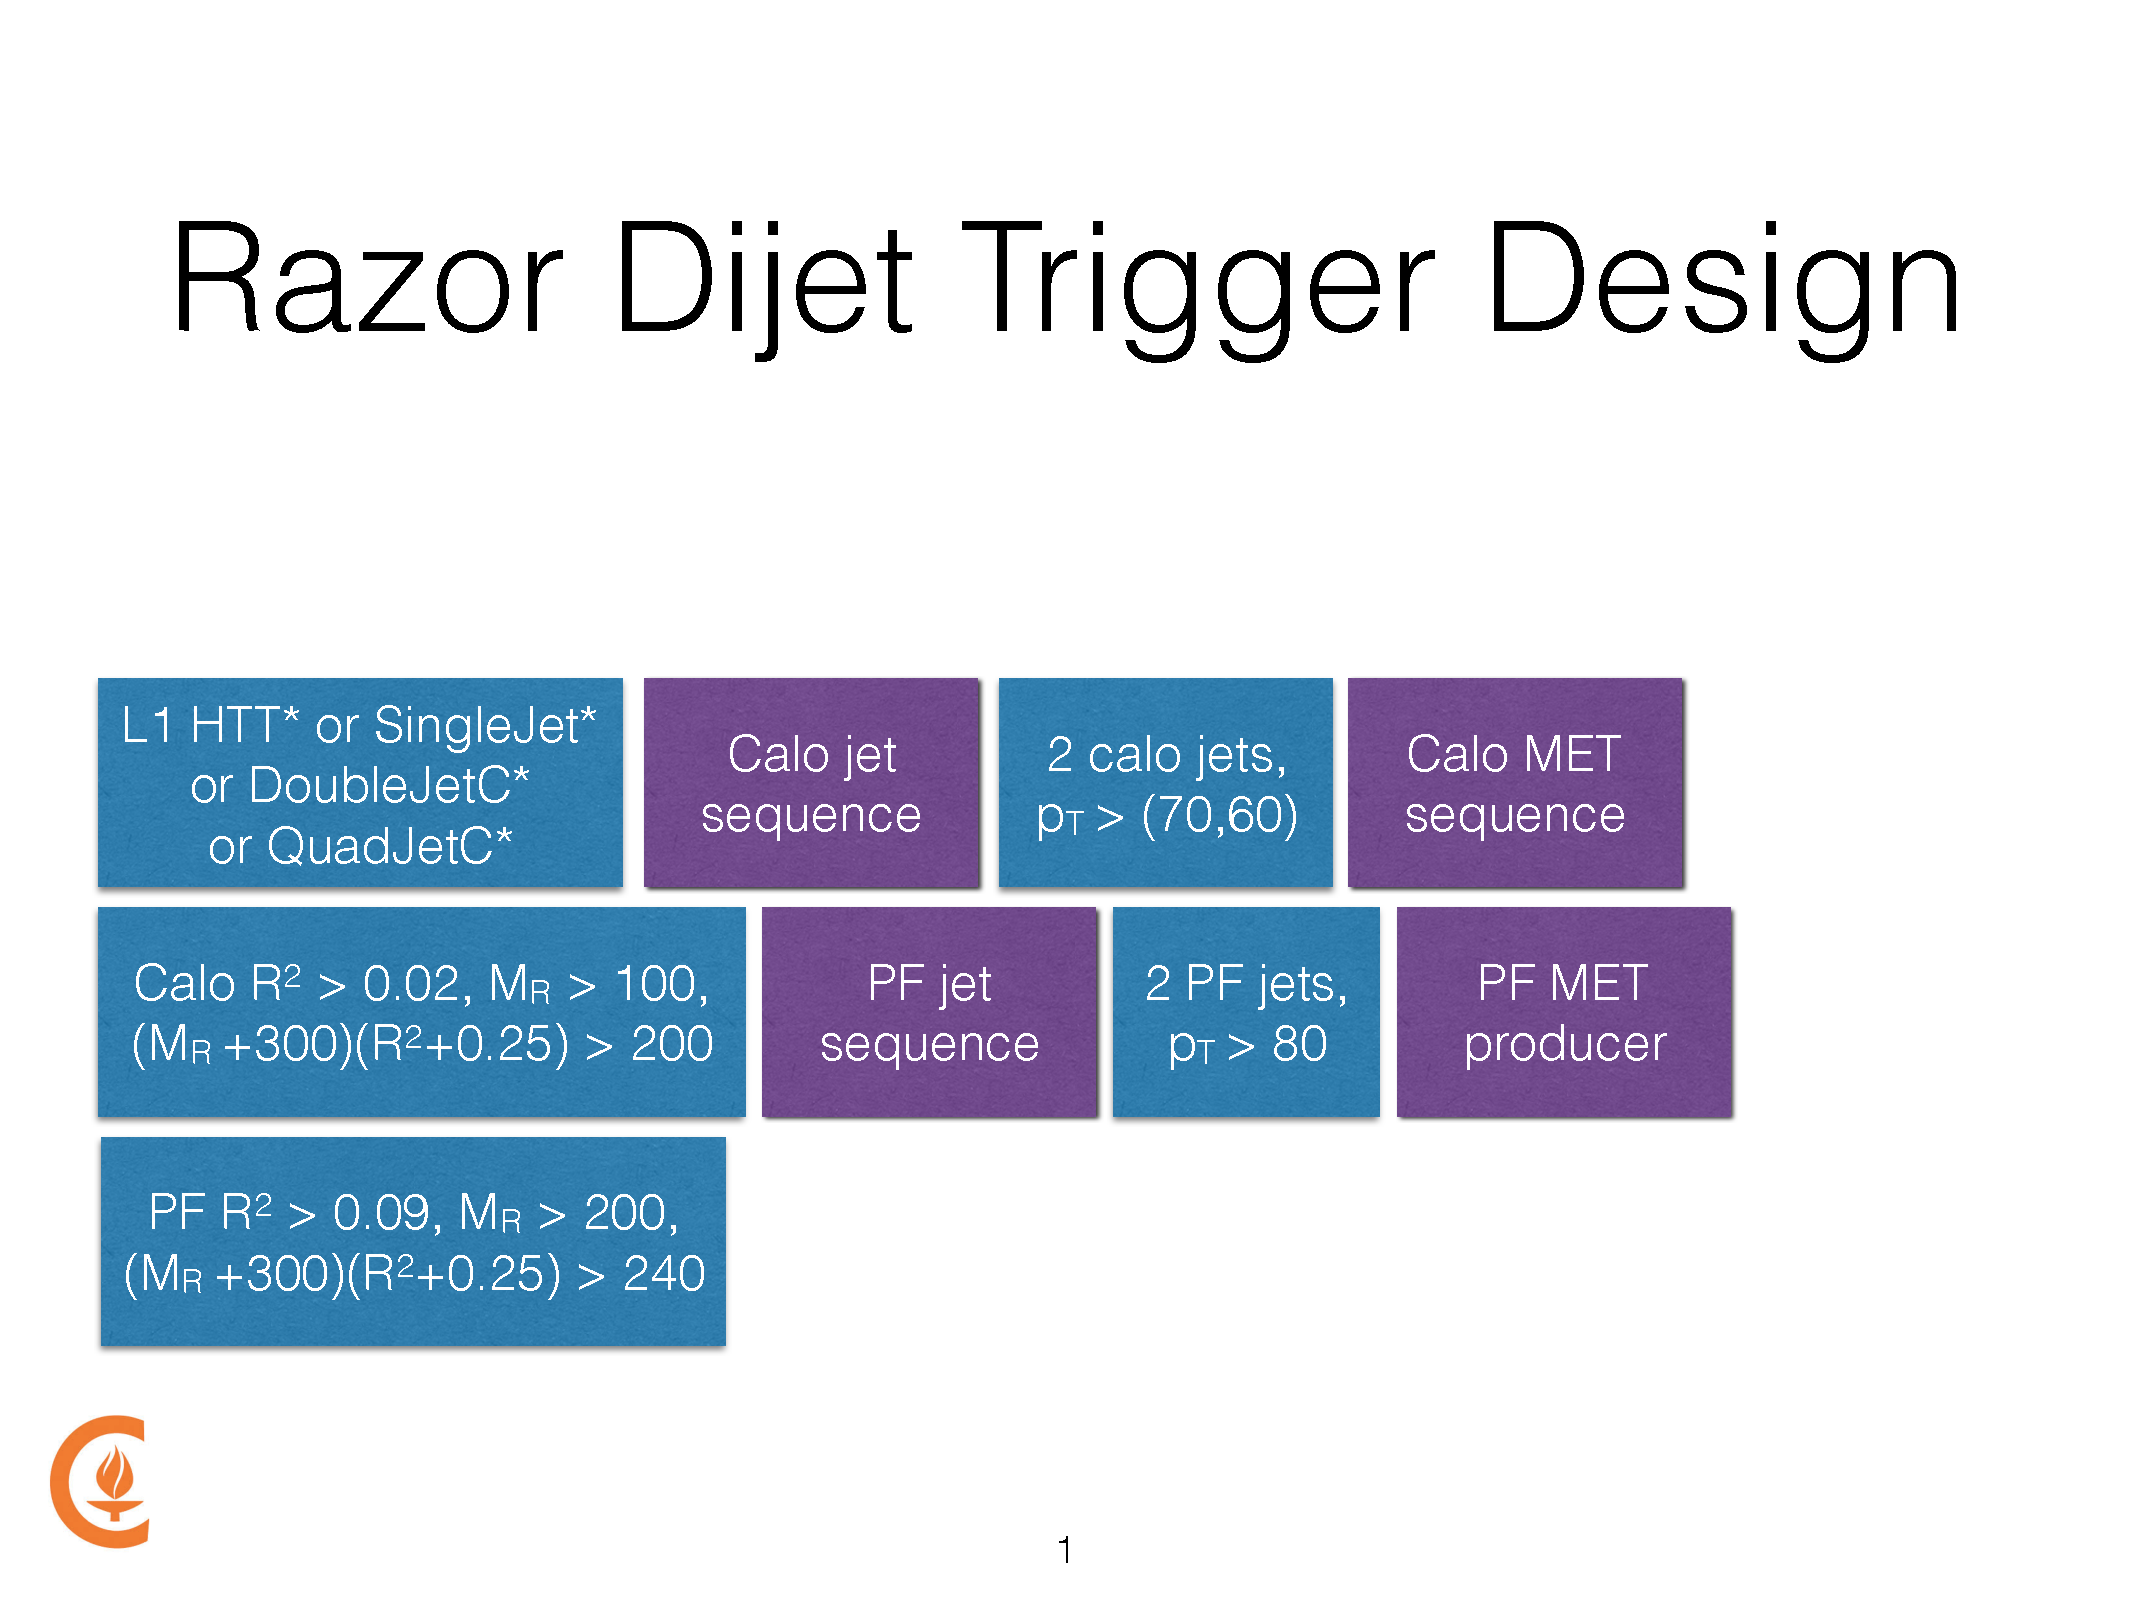
\includegraphics[width=0.8\textwidth,clip=true,viewport=0 110 1024
500]{figs/hlt13TeV/HLTDijetDesign.pdf}\\
(a) HLT\_RsqMR240\_Rsq0p09\_MR200 \\
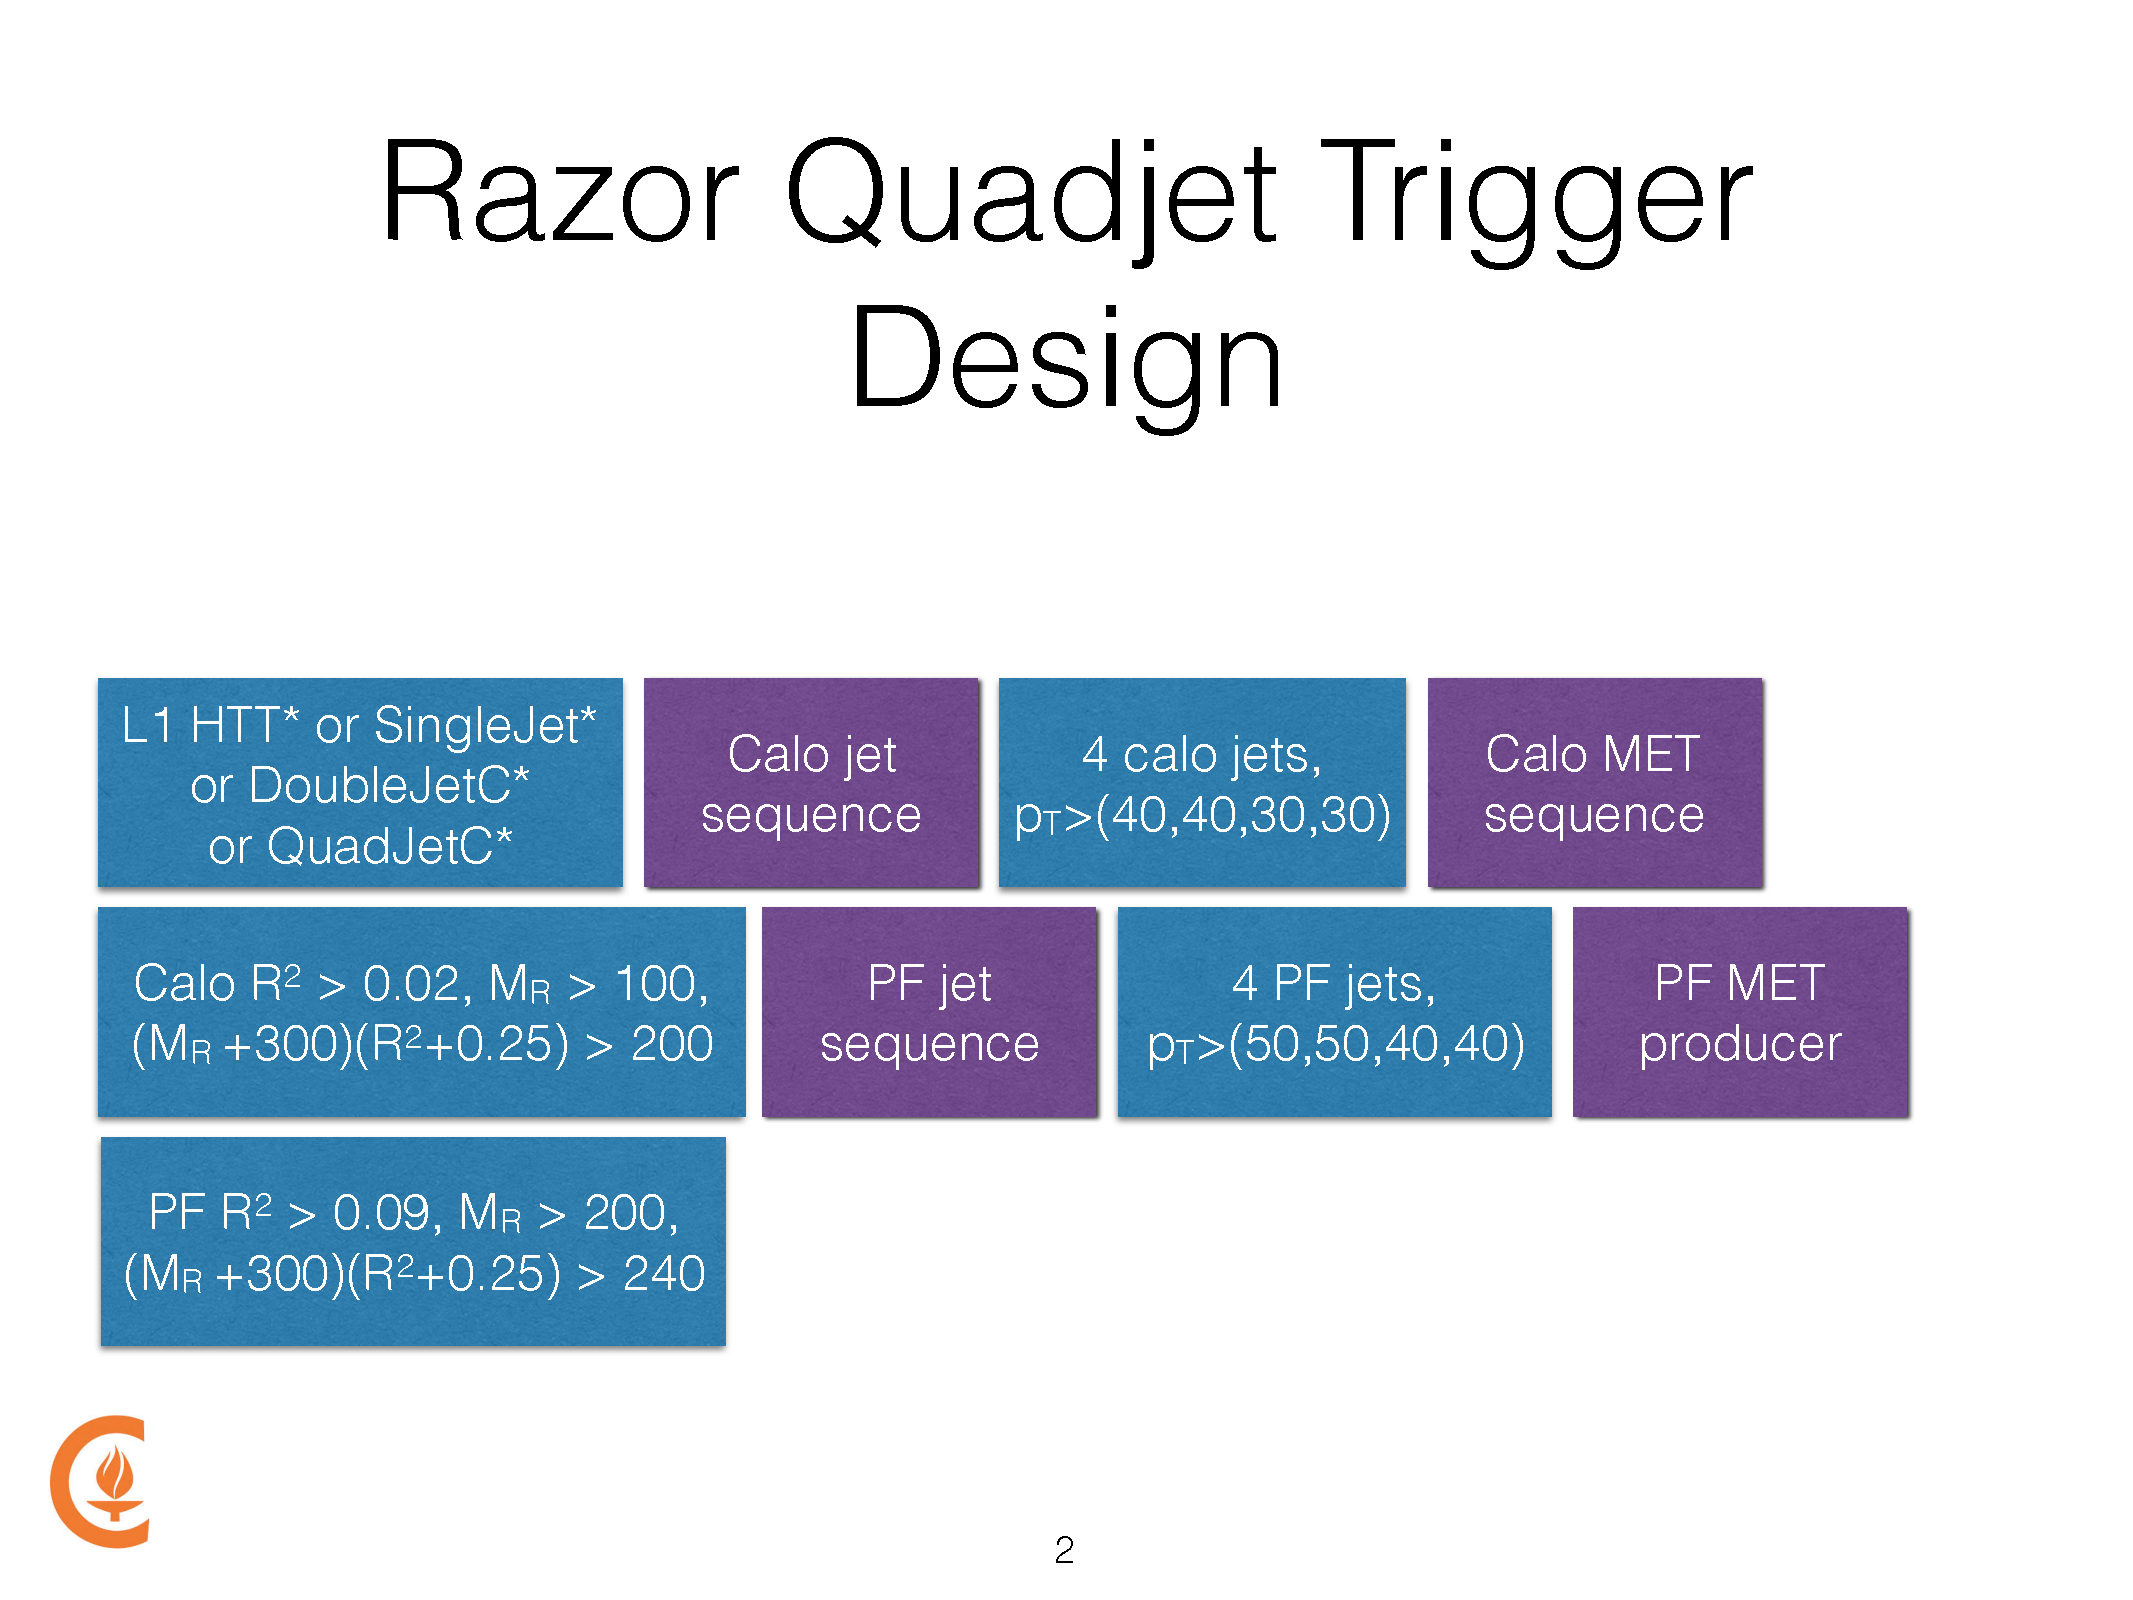
\includegraphics[width=0.8\textwidth,clip=true,viewport=0 110 1024
500]{figs/hlt13TeV/HLTQuadjetDesign.pdf}\\
(b) HLT\_RsqMR240\_Rsq0p09\_MR200\_4jet \\
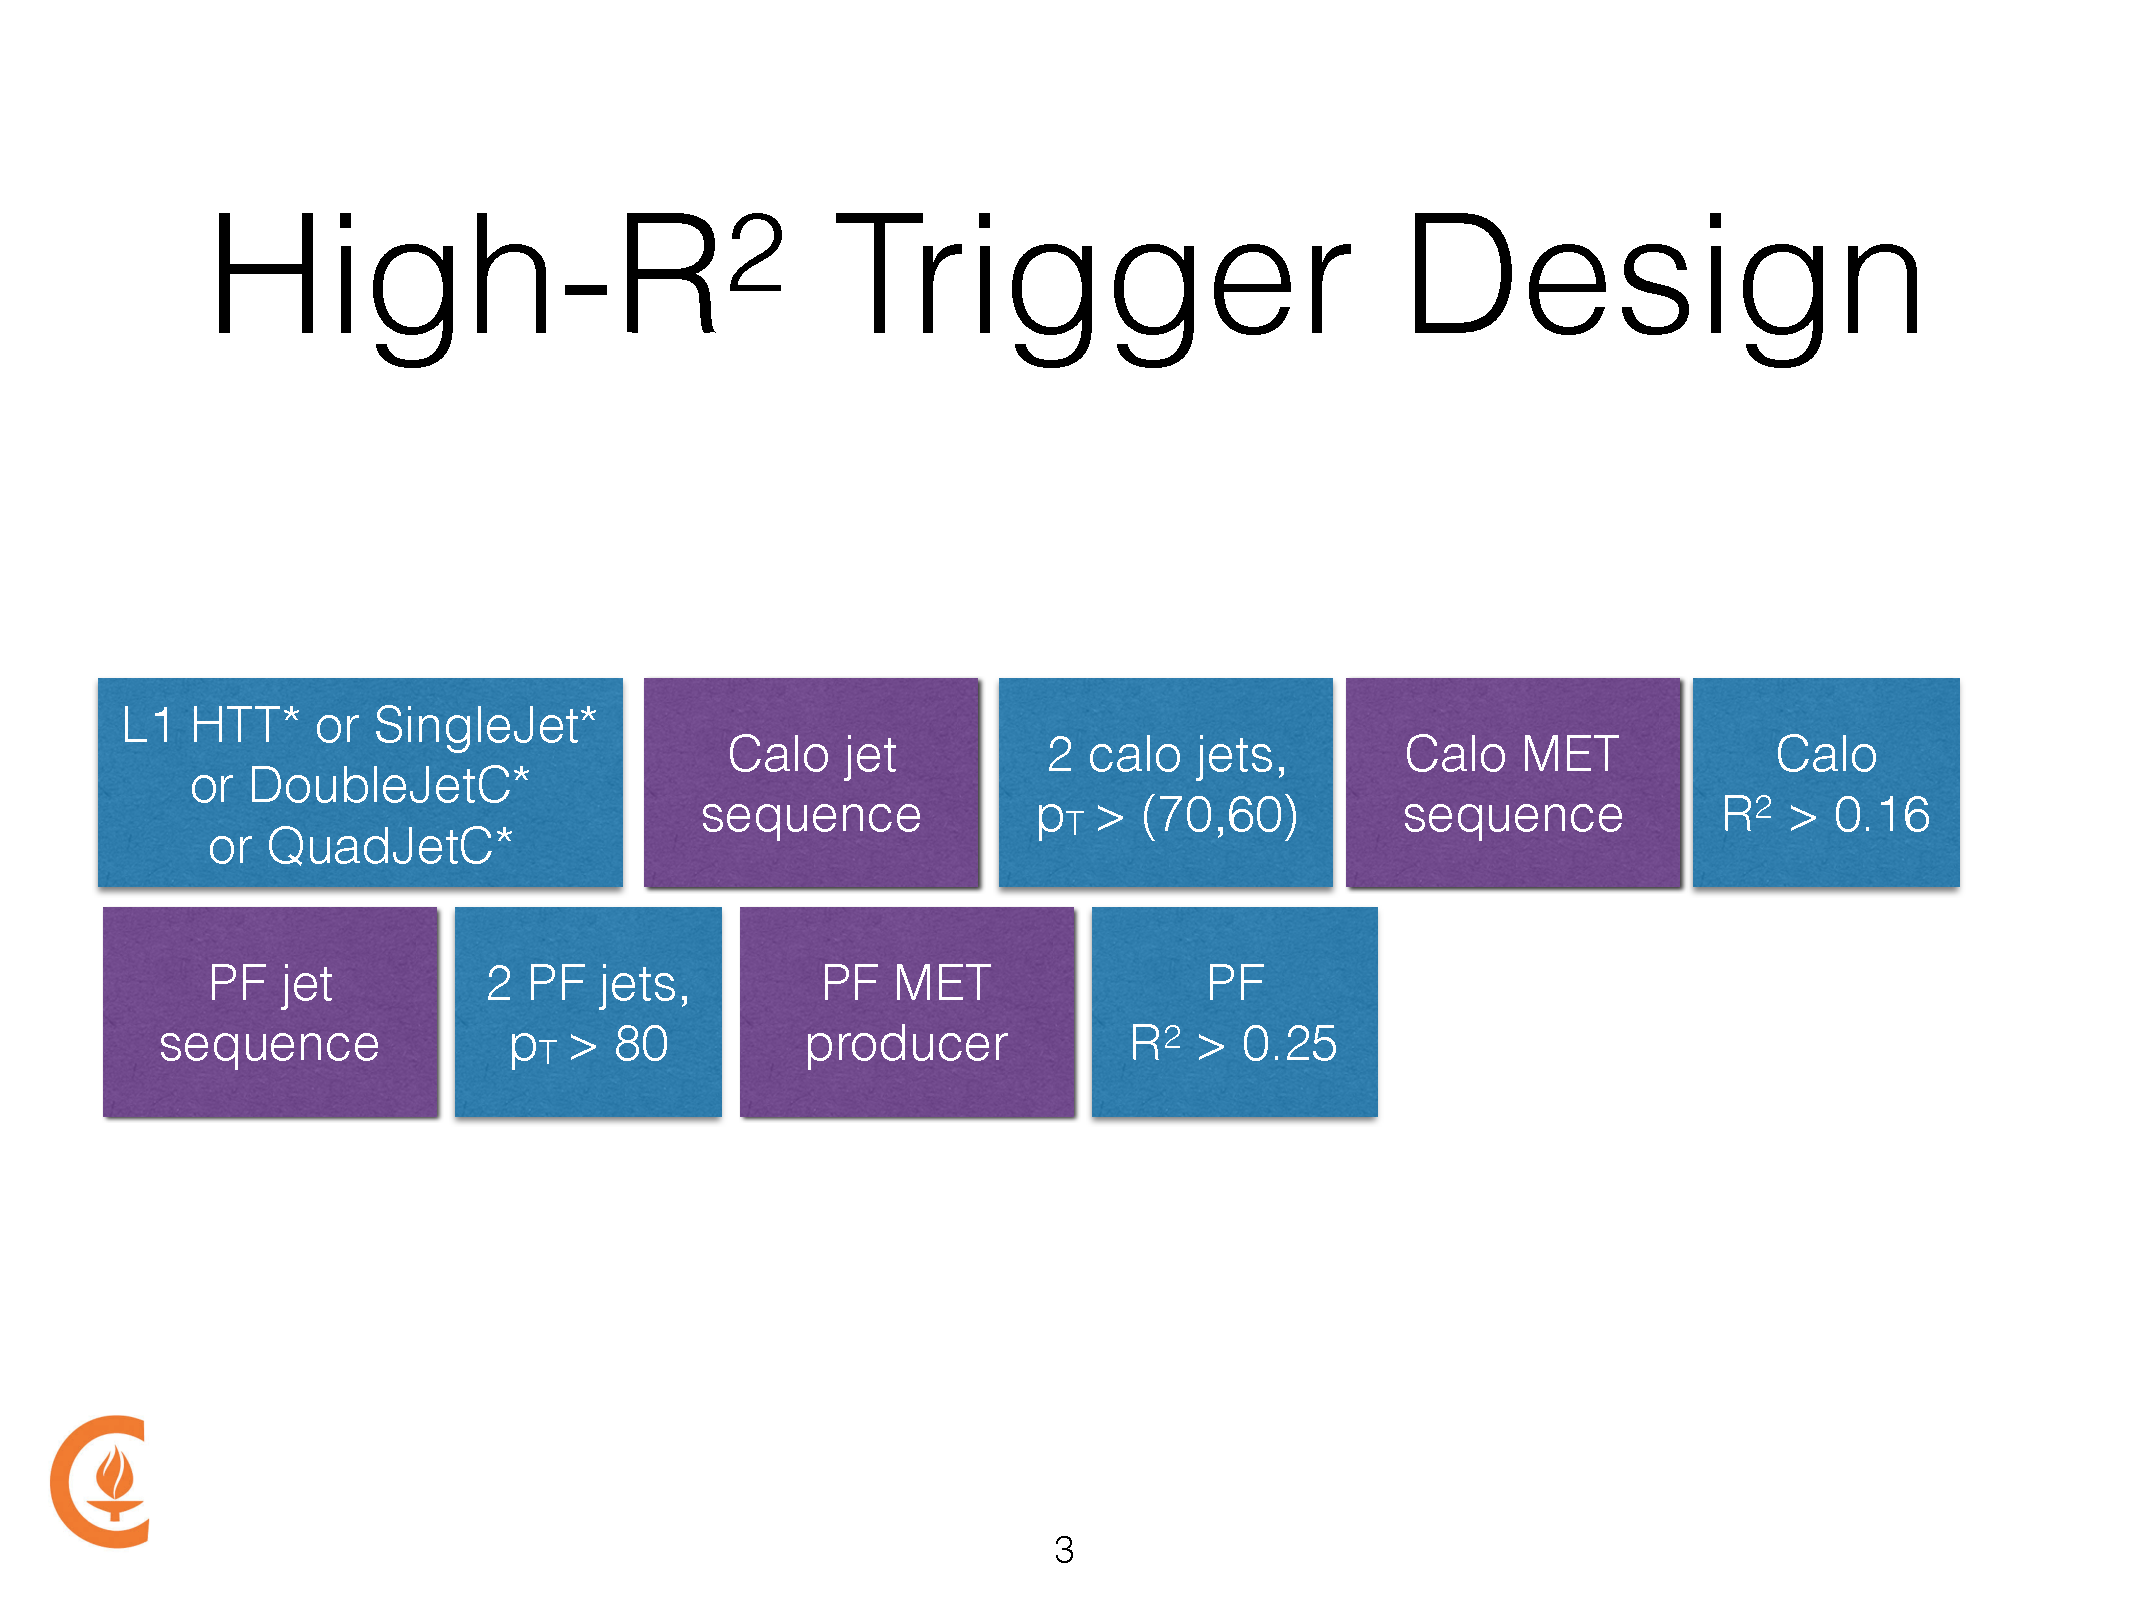
\includegraphics[width=0.8\textwidth,clip=true,viewport=0 220 1024
500]{figs/hlt13TeV/HLTR2Design.pdf}\\
(c) HLT\_Rsq0p25\\
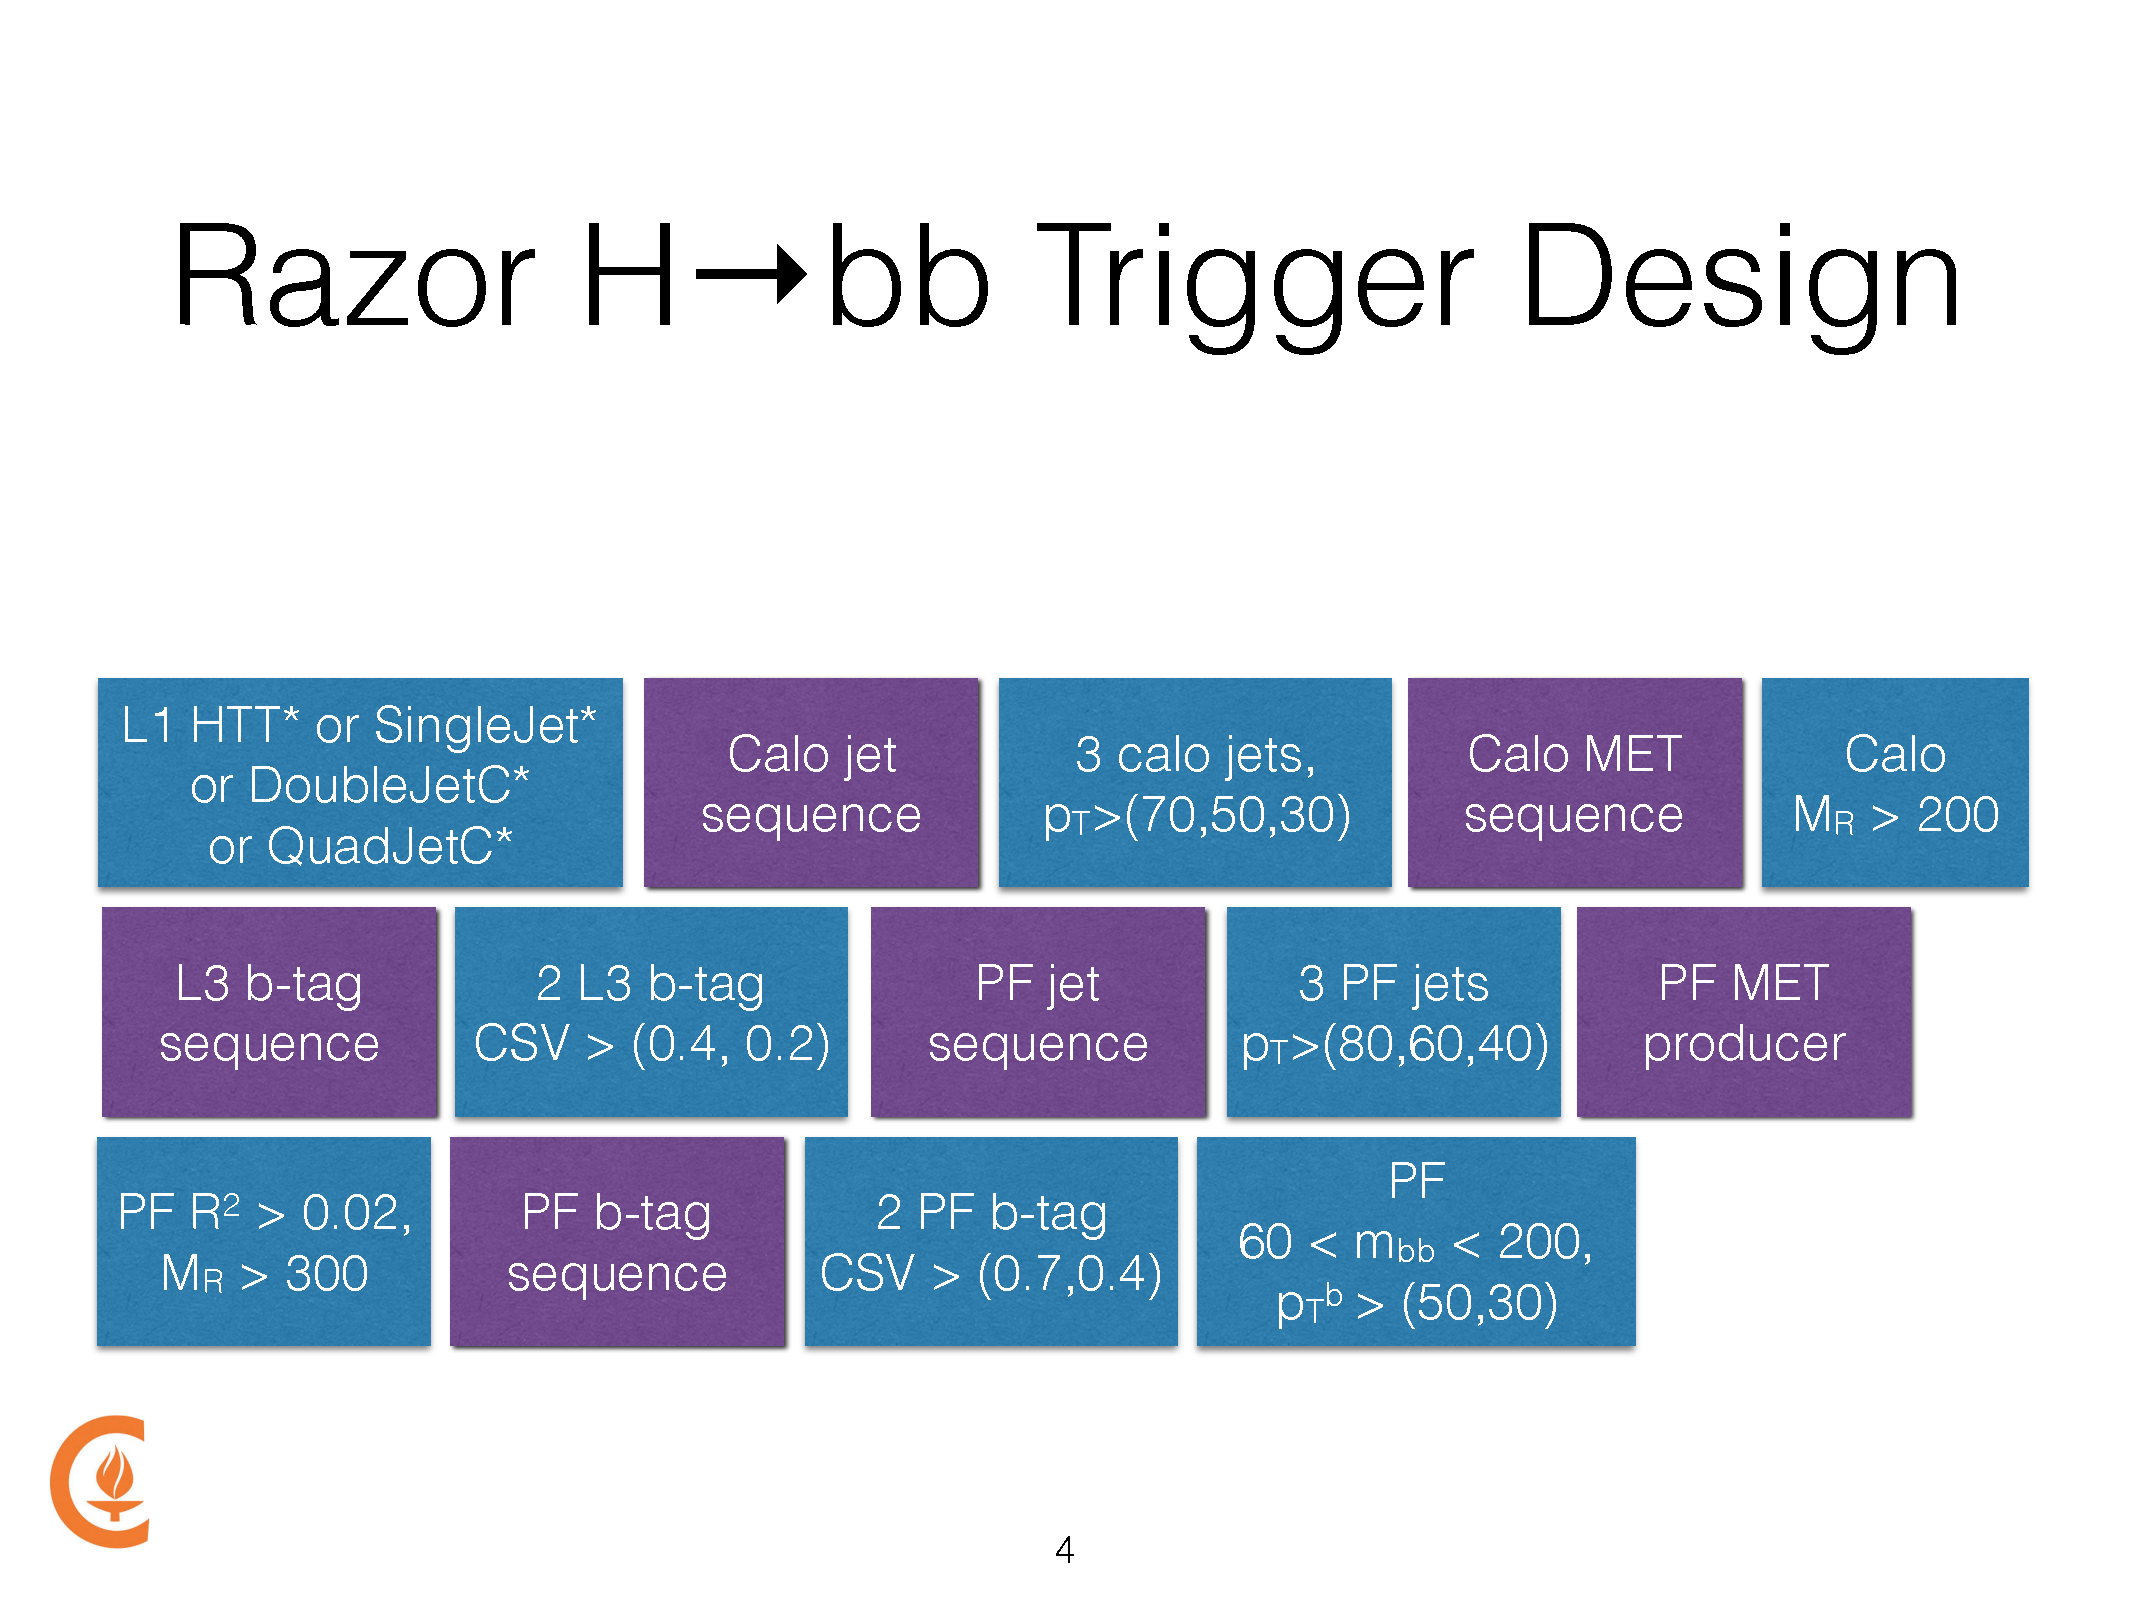
\includegraphics[width=0.8\textwidth,clip=true,viewport=0 110 1024
500]{figs/hlt13TeV/HLTRazorHbbDesign.pdf}\\
(d) HLT\_Rsq0p02\_MR300\_TriPFJet80\_60\_40\_\\
~DoublePFBTagCSV0p7\_0p4\_Mbb60\_200
\caption{\label{fig:HLTdesign} Flow of the producer steps (in purple)
  and filter steps (in blue) in
  the razor triggers~\cite{jmgd}.}
\end{figure}

\section{HLT rate and average CPU time}

The HLT rates and average CPU time consumed per event for the both the main and
backup razor triggers, as measured in data collected in 2015, are
presented in Tab.~\ref{tab:rates2015}. The thresholds on the razor
variables, jet $\pt$, and \cPqb-tag discriminator values, and were all
optimized to achieve an acceptable level of added rate and added CPU
time per event with respect to the rest of HLT menu (taking into
account overlapping events and reused algorithms) for the full suite of razor triggers. 

%\begin{table*}[ht!]
%\centering
% \caption{Rates for 0\unit{T} triggers.
% \label{tab:rates0T}}
%\resizebox{\textwidth}{!}{
%\begin{tabular}{l|l|l}
%\multirow{2}{*}{Trigger path} &  Data rate (run 260039) & MC rate (Spring '15) \\
% &  $4\times 10^{33}$ \unit{cm$^{-2}$ s$^{-1}$}, 17 PU &  \\\hline
%HLT\_Rsq0p25\_Calo & 3.7 Hz & \\
%HLT\_RsqMR240\_Rsq0p09\_MR200\_4jet\_Calo & 5.6 Hz & \\
%HLT\_RsqMR240\_Rsq0p09\_MR200\_Calo & 18.2 Hz & 
%\end{tabular}}
%\end{table*}

\begin{table*}[ht!]
\centering
 \caption{HLT rates and average CPU time consumed for the main and
   backup razor triggers under different running conditions in 2015. Run 260627 had $5\times 10^{33}$ cm$^{-2}$
   s$^{-1}$ peak instantaneous luminosity with 17 average pileup
   interactions, while run 259721 had $1.5\times 10^{33}$ cm$^{-2}$
   s$^{-1}$ peak instantaneous luminosity with 23 average pileup interactions. \label{tab:rates2015}}
\resizebox{\textwidth}{!}{
\begin{tabular}{l|c|c}
\hline\hline
\multirow{4}{*}{Trigger path} &  Data rate [Hz] & CPU time [ms]\\
& Run 260627 & Run 259721\\
 &  $5\times 10^{33}$ cm$^{-2}$ s$^{-1}$ &  $1.5\times 10^{33}$
                                          cm$^{-2}$ s$^{-1}$ \\
& 17 PU  & 23 PU\\
\hline
HLT\_RsqMR240\_Rsq0p09\_MR200 & 7.7 & 27 \\ 
HLT\_RsqMR270\_Rsq0p09\_MR200 & 2.3 & 17  \\ 
HLT\_RsqMR240\_Rsq0p09\_MR200\_4jet & 1.2 & 20 \\
HLT\_RsqMR270\_Rsq0p09\_MR200\_4jet & 0.5 & 15 \\
HLT\_Rsq0p25 & 0.7 & 14 \\
HLT\_Rsq0p30 & 0.4 & 14  \\
HLT\_Rsq0p02\_MR300\_TriPFJet80\_60\_40\_&\multirow{2}{*}{16.0} & \multirow{2}{*}{34}\\
~DoublePFBTagCSV0p7\_0p4\_Mbb60\_200 & &\\
HLT\_Rsq0p02\_MR300\_TriPFJet80\_60\_40\_ & \multirow{2}{*}{8.0} & \multirow{2}{*}{26}\\
~DoublePFBTagCSV0p7\_Mbb60\_200 & & \\
\hline\hline
\end{tabular}}
\end{table*}
% timing from: 
% https://docs.google.com/spreadsheets/d/1qu0dKZfjHEl073QyXayxzPBNoT10GZKMiPU9-z8VSeU/edit#gid=0
% supplemented by my measurement (for RsqMR240...)
% https://www.dropbox.com/s/z8qfx57du7h3gzq/TSG_RazorHLT2016_30Mar2016.pdf?dl=0


\section{Pileup dependence of HLT rate}
\label{sec:pileuphlt}
The HLT rate, normalized by the number of colliding bunches, as a function of the number of pileup interactions for
each razor trigger and for different data runs collected in 2015 is
shown in Figures~\ref{fig:HLTpileup1}~and~\ref{fig:HLTpileup2}. Nominally, the dependence of the
normalized HLT rate on pileup is expected to be linear, as is the case
for single-object triggers. In contrast, triggers based on sum quantities
(such as $H_\mathrm{T}$ or $\MET$) and multi-object triggers often
demonstrate a nonlinear dependence on pileup, not due to a physical
increase in the cross section of the selected physics processes, but rather due to the effects of pileup
contamination~\cite{Bocci:2016}. To illustrate this, consider the
case of a QCD dijet event with no true $\MET$. Normally such an event
would be rejected by $\MET$ triggers that require $\MET$ above some
threshold, but if some jets from pileup interactions are misinterpreted as part of the
event-of-interest then the HLT-reconstructed $\ptvecmiss$ will be
$-\sum_{j\in\mathrm{pileup}} \vecpt^{\,j}$, which may not perfectly balance to
zero as illustrated in Fig.~\ref{fig:pileupjet}.

\begin{figure}[ht!]
\centering 
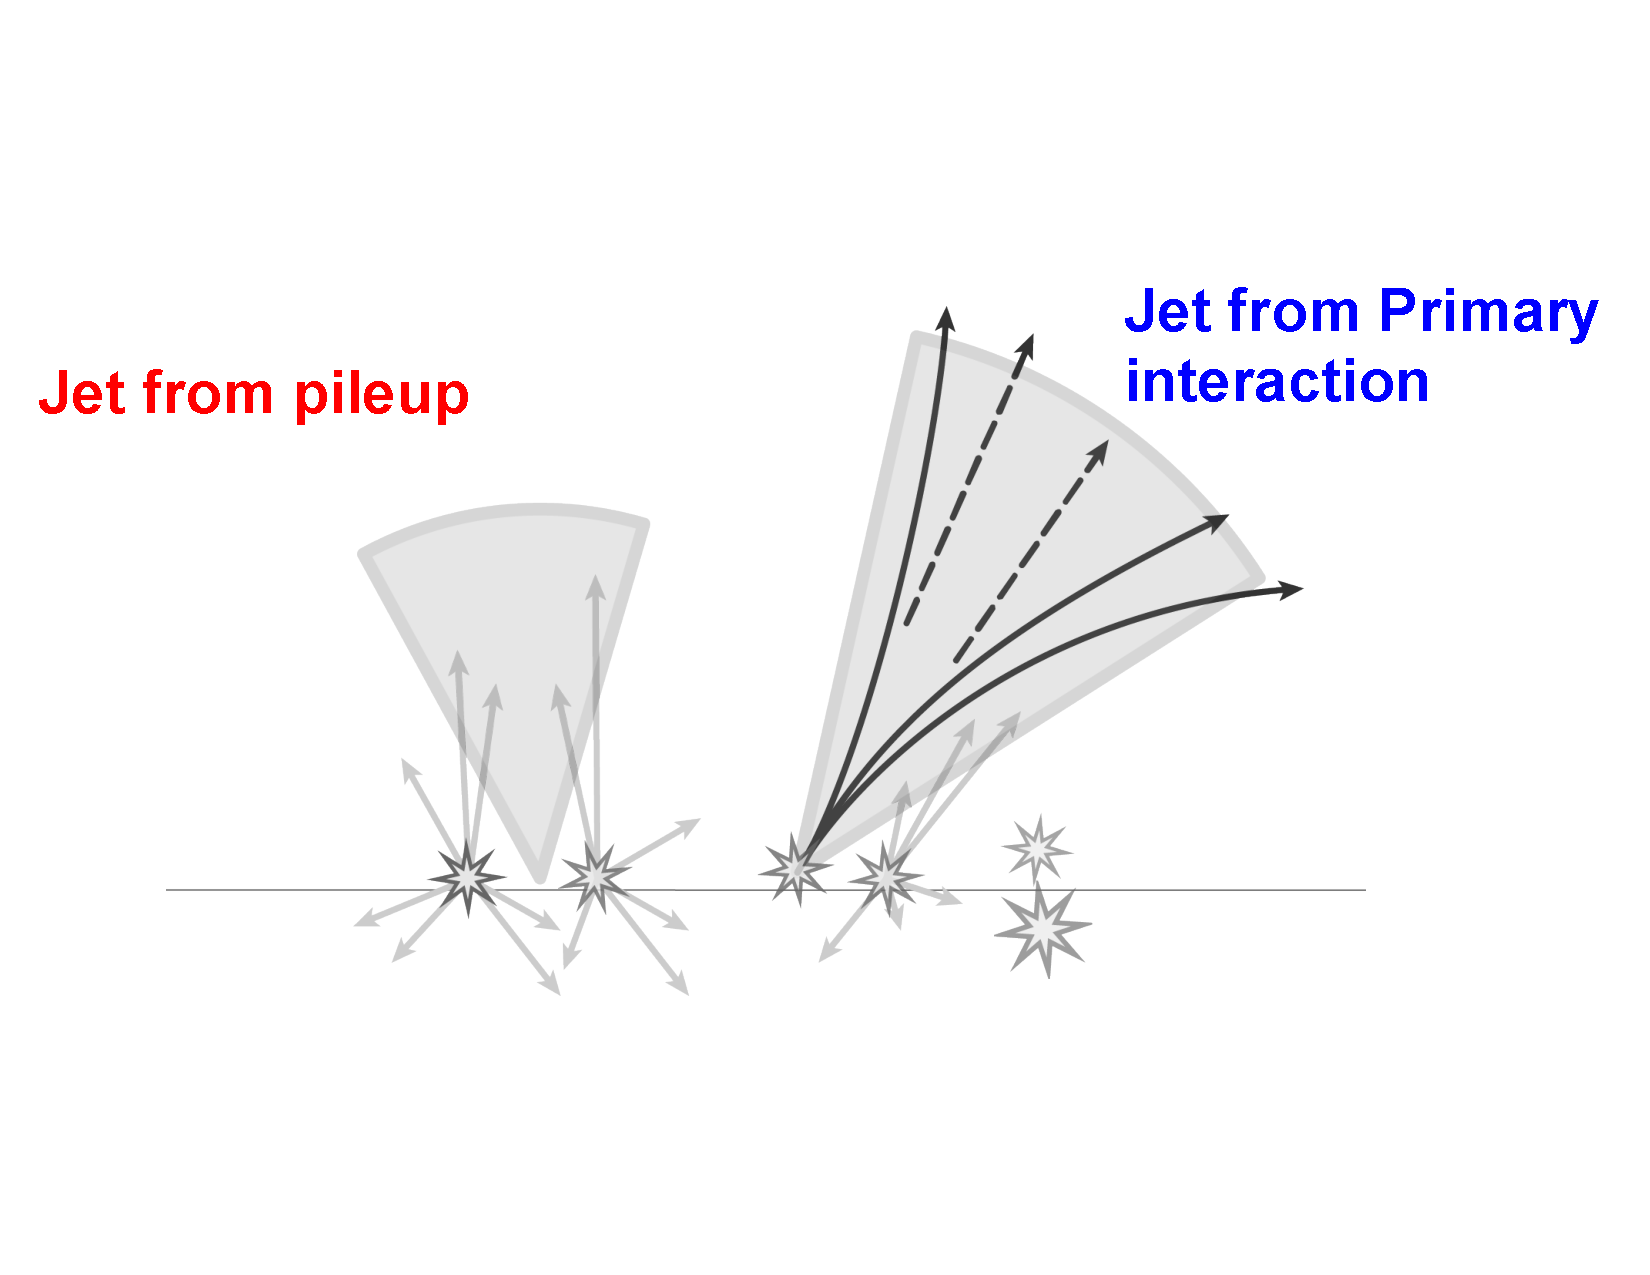
\includegraphics[width=0.7\textwidth]{figs/hlt13TeV/pileupjet.pdf}
\caption{\label{fig:pileupjet} Pileup jet misinterpreted as part of
  the main interaction event~\cite{jmgd}.}
\end{figure}

As the razor triggers are both based on sum quantities and multiple objects,
they also exhibit some nonlinear dependence on pileup. This implies
that as the pileup increases at the LHC in 2016 and beyond, either trigger thresholds
will need to rise dramatically or more sophisticated methods to deal
with pileup contamination will need to implemented. One such method is
delineated in Ch.~\ref{ch:timing}.

\begin{figure}[ht!]
\centering 
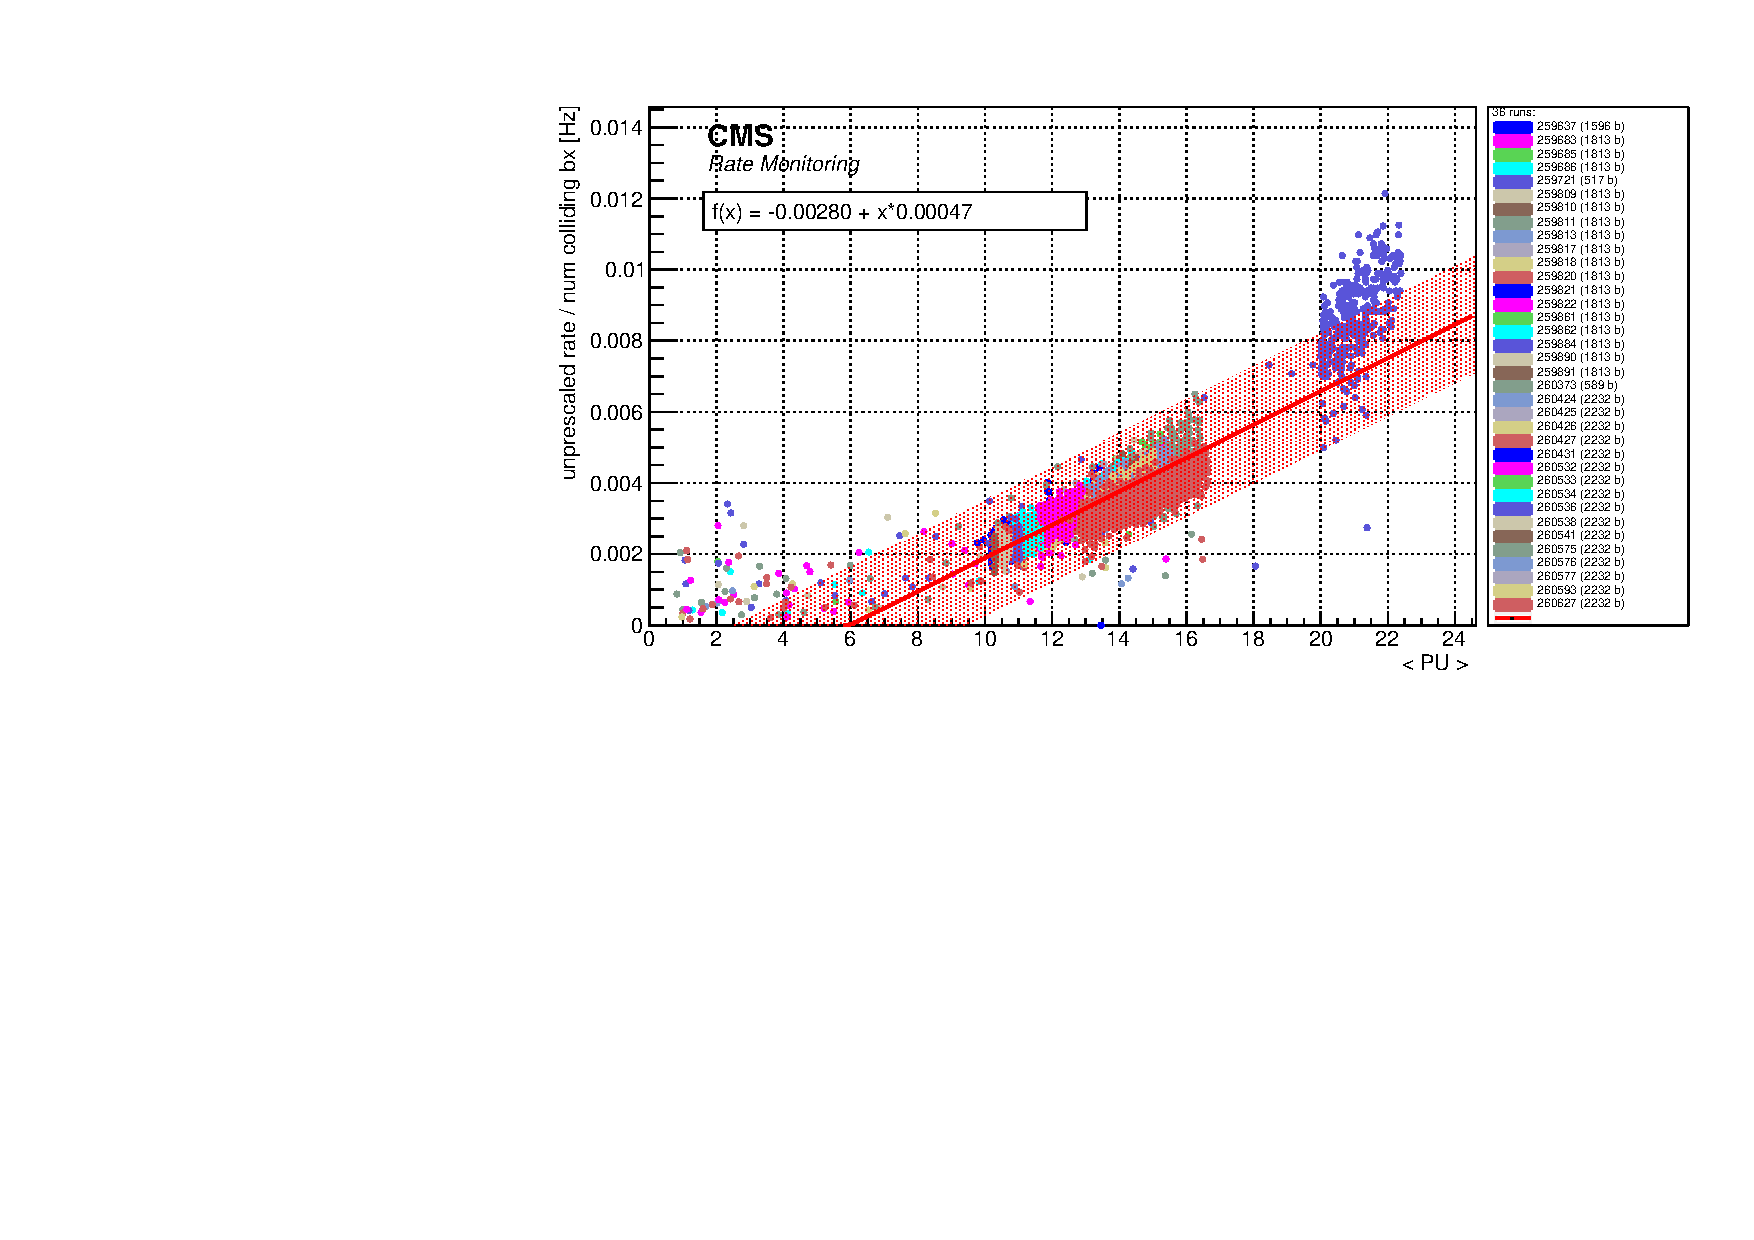
\includegraphics[width=0.9\textwidth]{figs/hlt13TeV/linear/HLT_RsqMR240_Rsq0p09_MR200_instLumi_vs_rawRate.pdf}\\
(a) HLT\_RsqMR240\_Rsq0p09\_MR200 \\
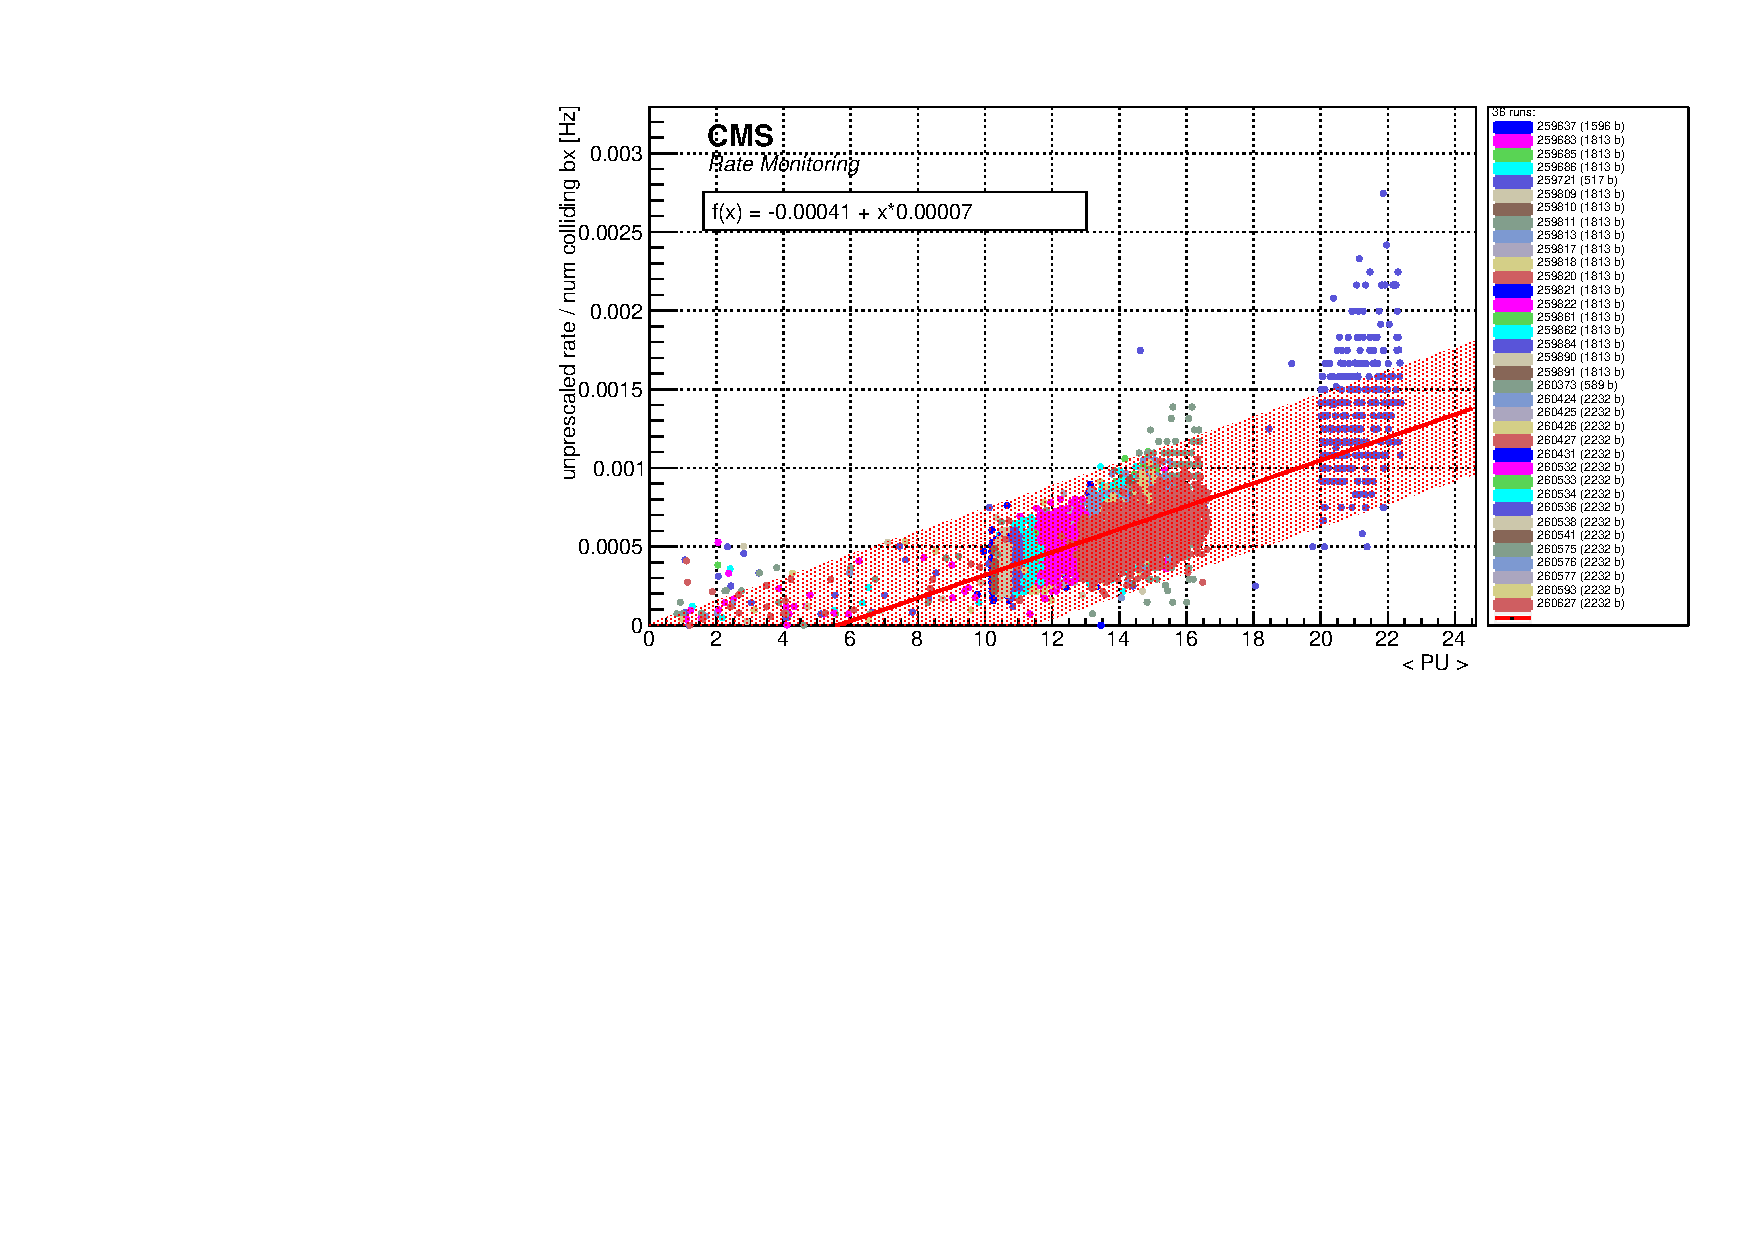
\includegraphics[width=0.9\textwidth]{figs/hlt13TeV/linear/HLT_RsqMR240_Rsq0p09_MR200_4jet_instLumi_vs_rawRate.pdf}\\
(b) HLT\_RsqMR240\_Rsq0p09\_MR200\_4jet
\caption{\label{fig:HLTpileup1} Pileup dependence of the dijet (a) and
  quadjet (b) razor triggers throughout 2015~\cite{jmgd}. Each data point
  corresponds to a different luminosity section (23.3 seconds of data-taking). The legend denotes the
  run number and number of colliding bunches in each run.}
\end{figure}

\begin{figure}[ht!]
\centering 
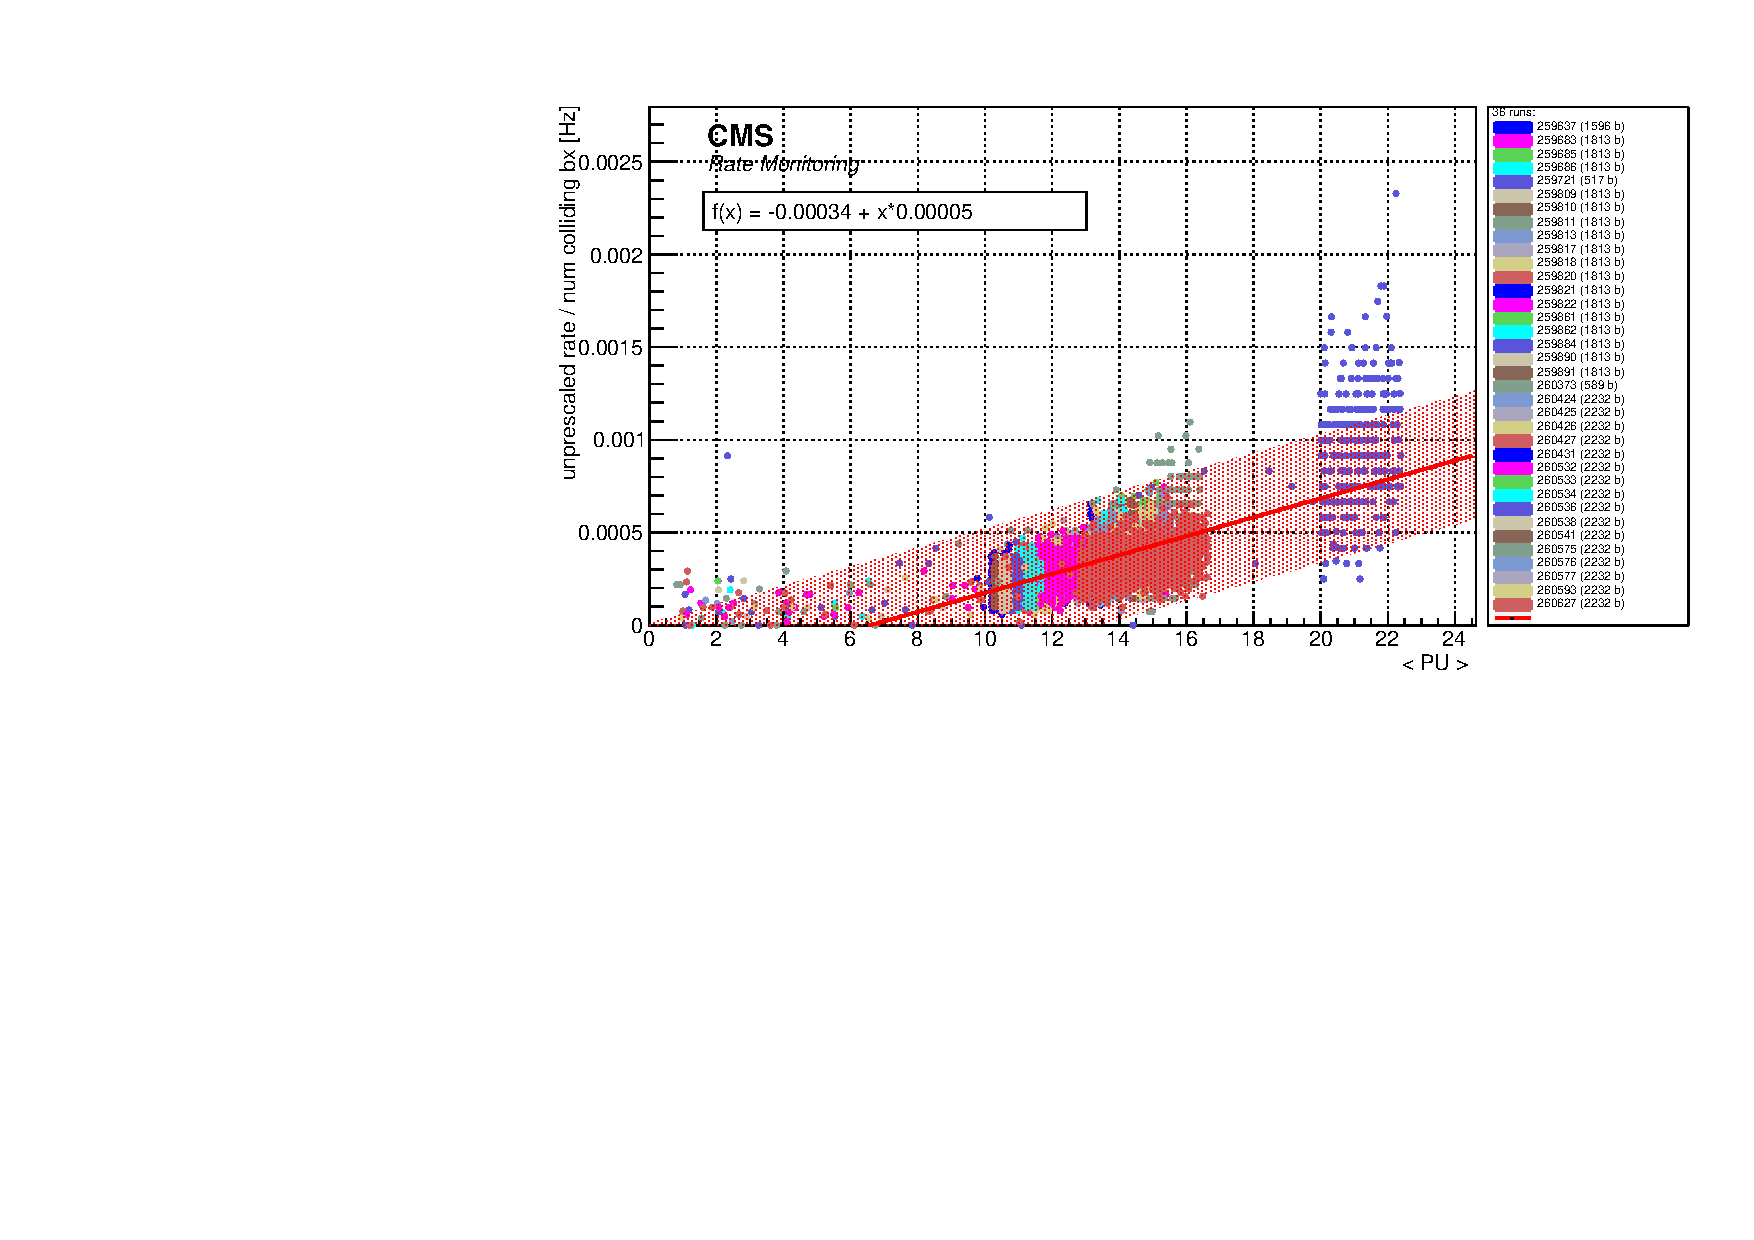
\includegraphics[width=0.9\textwidth]{figs/hlt13TeV/linear/HLT_Rsq0p25_instLumi_vs_rawRate.pdf}\\
(c) HLT\_Rsq0p25\\
 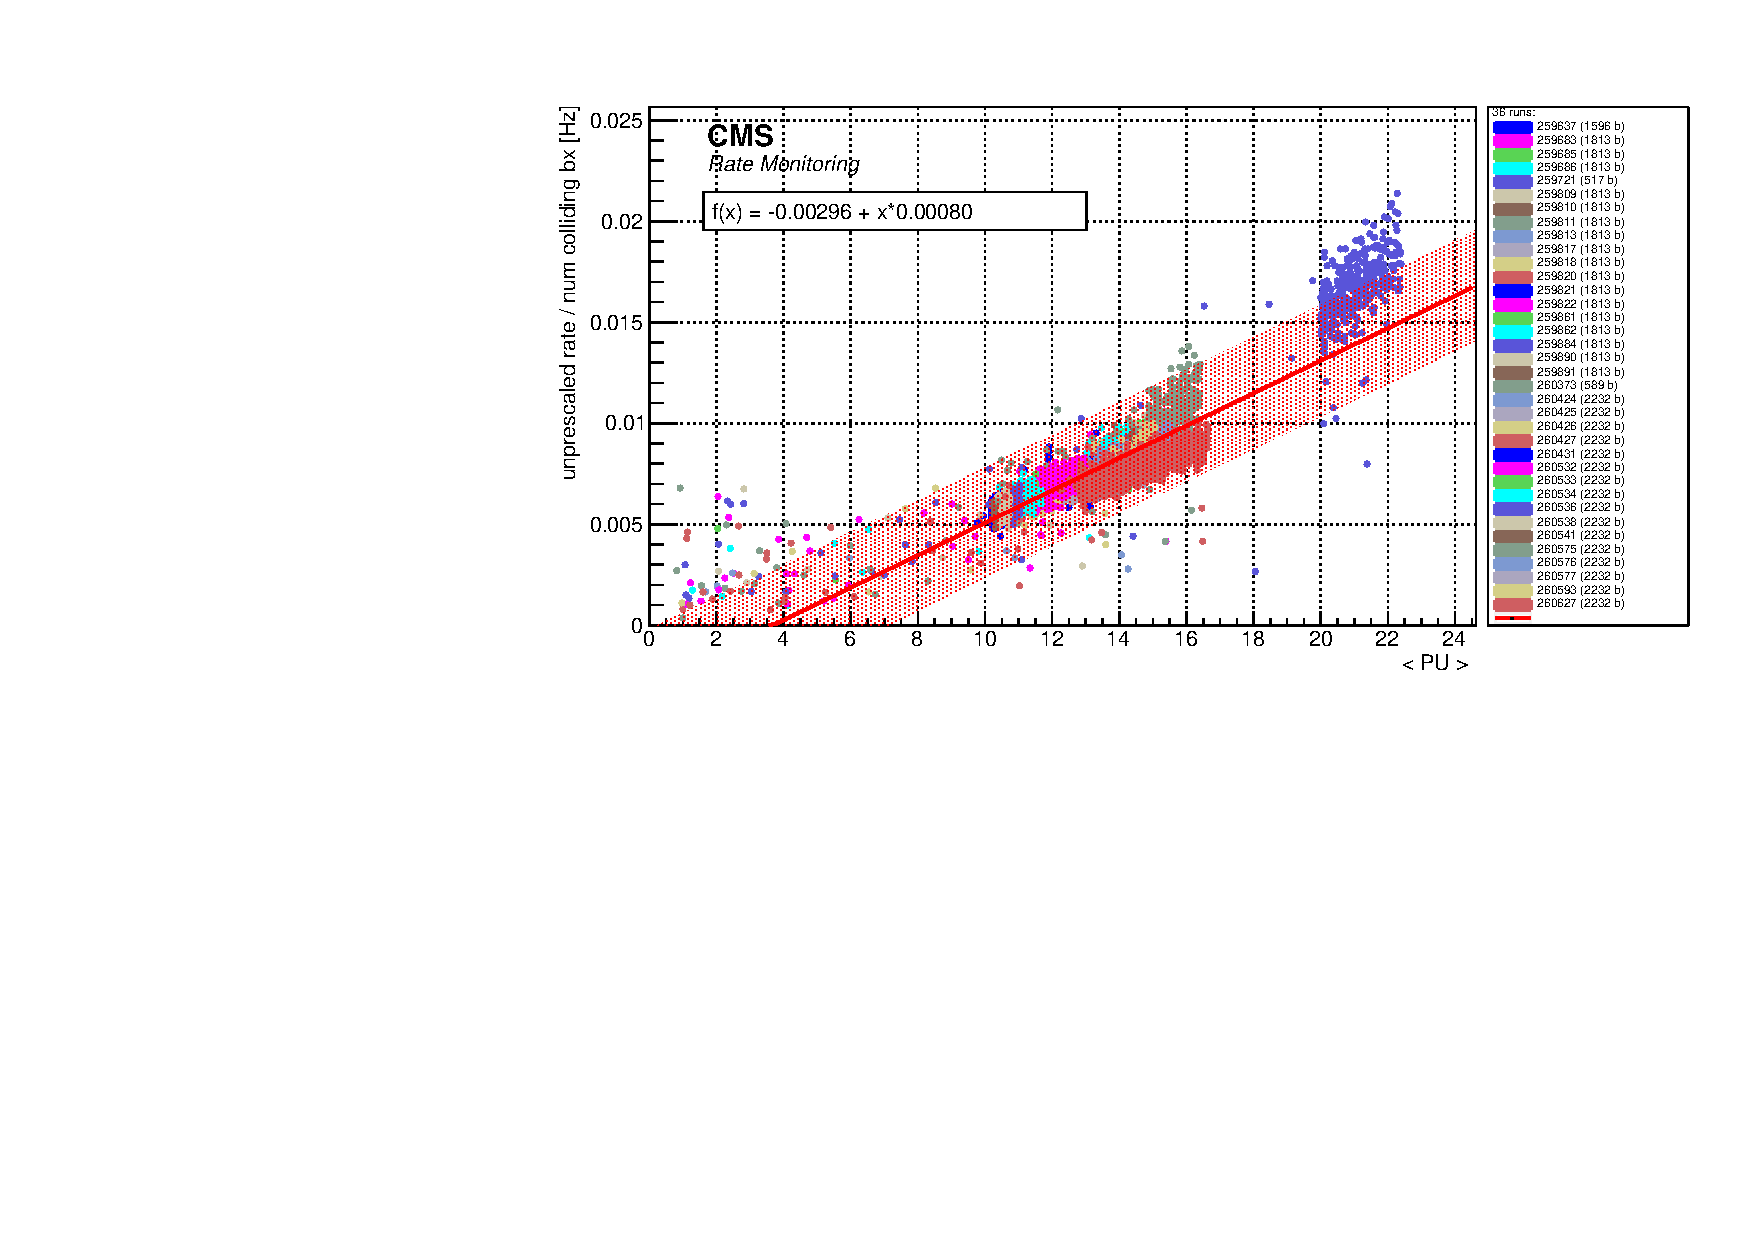
\includegraphics[width=0.9\textwidth]{figs/hlt13TeV/linear/HLT_Rsq0p02_MR300_TriPFJet80_60_40_DoublePFBTagCSV0p7_0p4_Mbb60_200_instLumi_vs_rawRate.pdf}\\
(d) HLT\_Rsq0p02\_MR300\_TriPFJet80\_60\_40\_\\
~DoublePFBTagCSV0p7\_0p4\_Mbb60\_200
\caption{\label{fig:HLTpileup2} Pileup dependence of the high-\Rtwo
  (c) and $\PH(\bbbar)$ (d) razor triggers~\cite{jmgd}. A detailed
  description of the graphs is given in Fig.~\ref{fig:HLTpileup1}}
\end{figure}


